\chapter{A SYSTEMATIC STUDY OF CRYPTOGRAPHIC FUNCTION IDENTIFICATION APPROACHES IN BINARIES}
\label{ch:cryptobinary}

\textit{This chapter is based on joint work with Christina Garman (Purdue University) along with Priyam Biswas (Intel) \footnote{Yongming Fan and Christina Garman's work was partially supported by NSF grant CNS-2047991.}. The paper was published in proceedings of the 2024 Annual Computer Security Applications Conference, pages 1092-1108 \cite{fan2024r+} \footnote{This paper also has an extended version presented at the 2024 Learning from Authoritative Security Experiment Results Workshop \cite{fanevaluating}.}.}

\section{Introduction}
%%%%%%%%%%%%%%%%%%%%%%

% Paragraph 1: why cryptographic functions are important
Cryptography has found itself at the core of secure modern technology and both plays a key role in securing communications and
is imperative to many modern systems and applications.
From data integrity to authentication and online banking to messaging friends, cryptography is everywhere.
Well-known cryptographic libraries, such as OpenSSL~\cite{openssl}, are widely used not only to generate
TLS certificates and validate certificate information, but also to implement cryptography in general purpose applications.
Despite their universal benign usage, cryptographic functions are also heavily used in malware and
to evade security protocols. In recent ransomware attacks ~\cite{wannacry,petya},
cryptographic functions have been used to encrypt a victim's information and later
asked to pay ransom in exchange of recovering their files and information.

% Paragraph 2: Motivation behind indentification 
On the one hand, the usage of cryptographic functions makes it easier to carry out
secure and private operations, and on the other hand, its malicious usage by bad actors makes
it harder for cryptography and security experts to perform forensic analyses and reverse engineer code.
Hence, the ability to automatically identify or detect the presence of cryptographic functions
in binary applications can be a crucial part of the security experts' arsenal.
It can assist in binary analysis to give a better depiction of how the
functions work.  Determining the type of cryptographic function in a
binary can help to pinpoint the existence of a malicious
payload~\cite{yan2008revealing} and also help cryptographic experts identify potentially insecure protocols or implementations (or those that require more manual analysis).
%Finally, oftentimes malware and ransomware use
%similar cryptographic functions with some minor changes. For example, there are
%different versions of the TeslaCrypt ransomware~\cite{teslacrypt}.
%Identifying one piece of ransomware via an automatic detection mechanism can help to
%identify other versions and thus save time and resources that could be better devoted to implementing
%effective prevention mechanisms.

\begin{figure}[t]
  \centering
  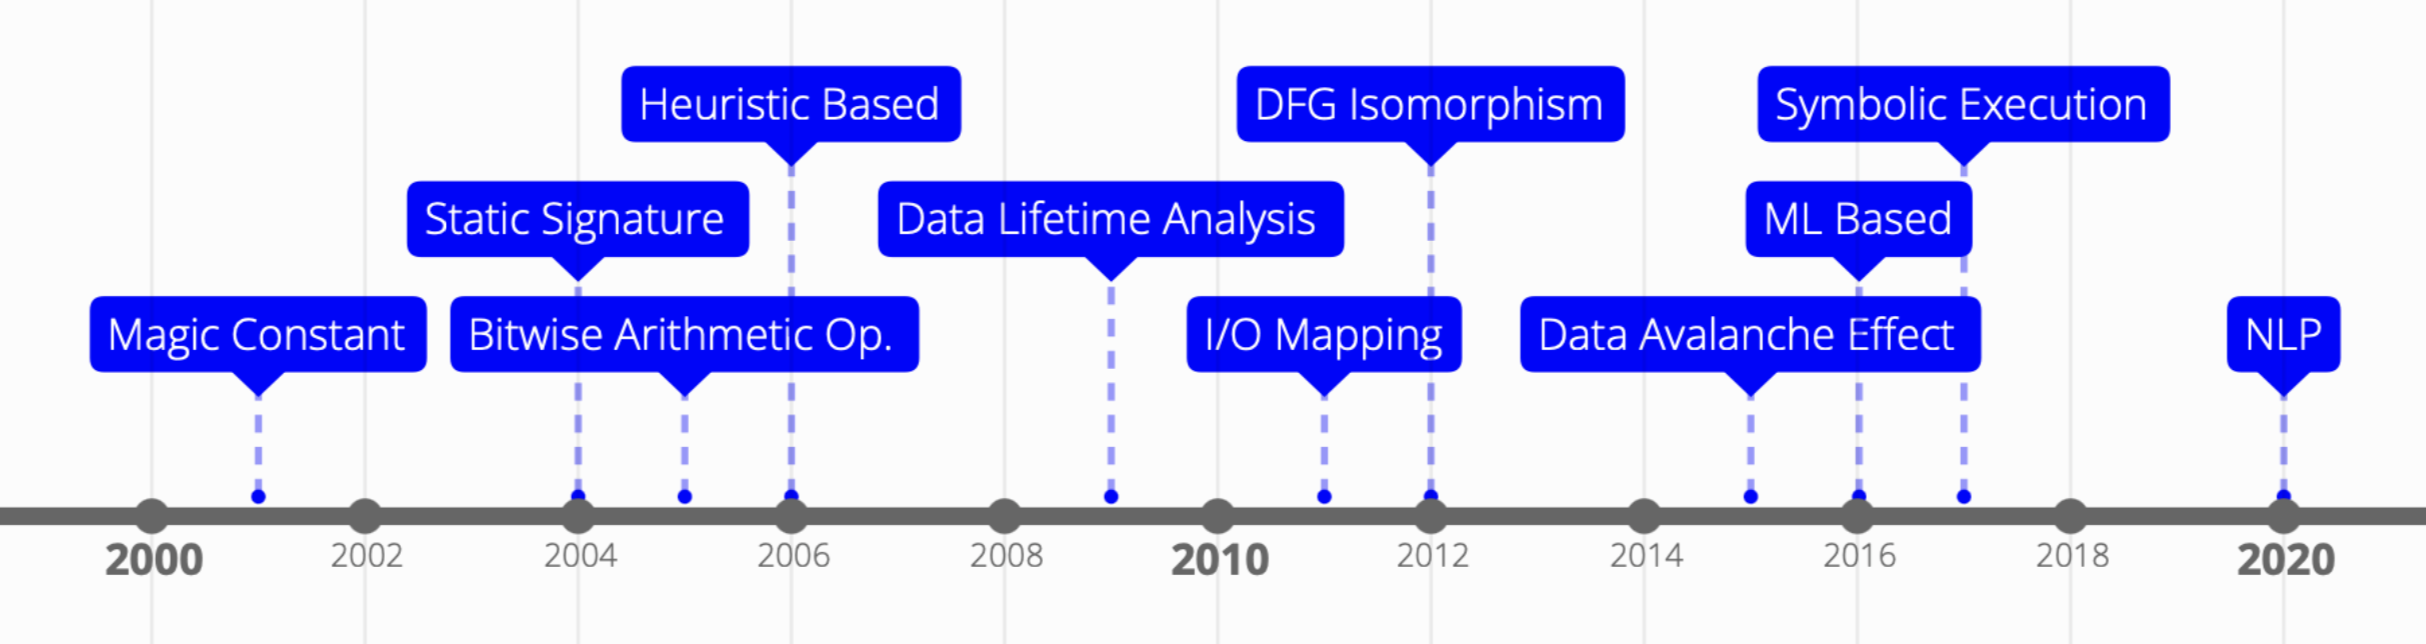
\includegraphics[width=0.95\textwidth,keepaspectratio]{ch-cryptobinary/figure/Crypto_timeline.png}
  \caption{Evolution of cryptographic function identification techniques}
  \label{fig:cryptobinary-timeline}
\end{figure}

%%4 Paragraph 3: Challenges
%However, cryptographic function identification has its own sets of challenges.
%Binaries can be obfuscated in a variety of ways, such as control-flow flattening,
%data-splitting, data-aggregation, and inclusion of bogus control-flow. In addition,
%simple cryptographic algorithms can be implemented in a variety of ways, hence
%detection mechanism that may work on one variation may fail on its more complicated (or more simplified) implementations. Malware authors also generate packed binaries to evade
%any possible detection.


While general purpose binary analysis and function identification techniques are themselves broad and thriving areas that could potentially solve these problems, a variety of work across industry and academia has focused on solving these challenges more specifically: developing techniques and tools that are uniquely tailored to identifying \textit{cryptographic primitives} in binary applications.  This allows researchers to often provide better results in different domains, leveraging cryptography-specific features.
% Paragraph 4: landscape
Cryptographic functions tend to have many mathematical computations,
nested loops, and exclusive input-output mappings which are distinct from
non-cryptographic functions and can thus be useful as a means of identification. 
% \autoref{fig:cryptobinary-timeline} shows a timeline of various techniques and approaches used in cryptographic function identification research to date.
%\priyam{taken it to the background}
Harvey et al.~\cite{harvey2001cipher} first utilized magic constants to identify
cryptographic primitives in 2001. Later works focused on signature
based detection mechanisms. However, due to the limitations of signature
based approaches, subsequent work placed a greater emphasis on heuristic based detection, such as
identification of basic blocks, instruction patterns, etc. With the
popularization of modern machine learning algorithms, newer works utilized
deep learning and AI to extract cryptographic features from a binary.
%We discuss these various approaches in depth in Section~\ref{sec:features}.

Unfortunately, while there has been a wealth of work in the space, it has generally failed to keep up with modern cryptographic
innovations and applications, as well as current software engineering and optimization techniques.
This can be difficult to notice as there is no standardized benchmarking or comparison framework, and individual works tend to test on algorithms that they are best at identifying, while neglecting those they cannot.
Additionally, as many techniques are tailored for specific cryptographic algorithms, architectures, or settings, which change rapidly over time, reproducing past results can be challenging, making it difficult to provide comparisons across the growing landscape as well.
%Additionally, while there have been some surveys on encryption algorithms~\cite{mushtaq2017survey} and ransomware detection/mitigation~\cite{begovic2023cryptographic, mcintosh2021ransomware, smith2022machine}, these works do not investigate the capabilities of different detection tools or the gaps in the selection of algorithms.

Given how important these tools and techniques can be for both researchers and practitioners, we aim to reproduce and replicate all existing tools to date in this domain.  In this endeavor, we also offer a comprehensive analysis that categorizes and discusses the existing body of work, highlighting the strengths, weaknesses, and techniques employed.
We also seek to help drive future research in the area by identifying potential challenges and various factors that may influence performance.
%highlighting a taxonomy of modern cryptographic algorithms and discussing features that we think could be leveraged for identification. 
To help provide for a more even comparison of existing and future work, and to identify gaps that are in need of future research, we create a benchmarking framework featuring a number of modern cryptographic primitives and applications. We then use this framework to evaluate existing work.
Finally, throughout the paper, we discuss and motivate a variety of open research problems in the space.

\subsection{Our Contributions}
Our primary contributions are:

\begin{itemize}[noitemsep,topsep=0pt]

%\item We present a systematic study of cryptographic function identification
%approaches, discussing various techniques that have been leveraged, as well as their strengths and weaknesses.

\item We conduct a thorough examination of cryptographic function identification methods, exploring the range of techniques utilized and evaluating their respective strengths and limitations.

%\item We highlight a taxonomy of modern cryptographic algorithms and discuss various features of cryptographic algorithms that can be leveraged for identification purposes.
%\item We highlight a number of features of cryptographic algorithms that can be leveraged for identification purposes.

%\item We discuss a number of challenges that modern tool developers and researchers face in the space from a software and implementation perspective, such as optimizations and non-standard implementations.

\item We create a standardized suite of performance metrics and benchmarks to evaluate the effectiveness
of current detection mechanisms and analyze existing tools based on this suite.

\item We conduct comprehensive replication and reproduction studies on all existing work.

\item We provide an in-depth analysis of our findings and categorize the tools according to their performance across various dimensions.

\item Based off of this analysis and our study of existing work, we discuss the research gaps in this domain and propose directions for future work.

%\item We propose a simple tool to identfy cryptographic functions based on the program state change \priyam{TODO: update based on the eval status}
  
%\item We present a comprehensive framework to understand the scalability and
%impact of dynamic analysis in detection mechanisms. \clg{Is this one left over from your thesis?  I'm not sure how it fits in overall with the paper.}
%\priyam{we can get rid of this part}

\end{itemize}

% \subsection{Chapter Organization} The outline of our paper is as follows.
% In Section~\ref{sec:taxonomy} we present our taxonomy of cryptographic algorithms, and in Section~\ref{sec:features} we discuss the various features of cryptographic algorithms that have been used for identification.
% In Section~\ref{sec:detection} we analyze different detection techniques and their strengths and weaknesses, and in Section~\ref{sec:challenges} we enumerate the inherent challenges in detecting and classifying cryptographic code in real-world applications.
% In Sections~\ref{sec:framework} and~\ref{sec:evaluation} we introduce our benchmarking framework and run existing tools on it to generate a fair comparison among existing work and highlight gaps in coverage.


\section{Background}
\label{sec:cryptobinary-background}
%%%%%%%%%%%%%%%%%%%%

In this section, we provide background on and a classification of detection approaches that have been employed by existing tools to date.
%To our surprise, only a limited number of tools and approaches have been developed throughout the span of more than two decades.
\autoref{fig:cryptobinary-timeline} shows the evolution timeline of various techniques and approaches used in cryptographic function identification research whereas \autoref{fig:cryptobinary-tool_timeline} shows the development timeline of all studied tools.
We also provide an overview of some of the cryptographic features that existing tools focus on, to help better understand how they work and contextualize later discussion.

\begin{figure}[t]
  \centering
  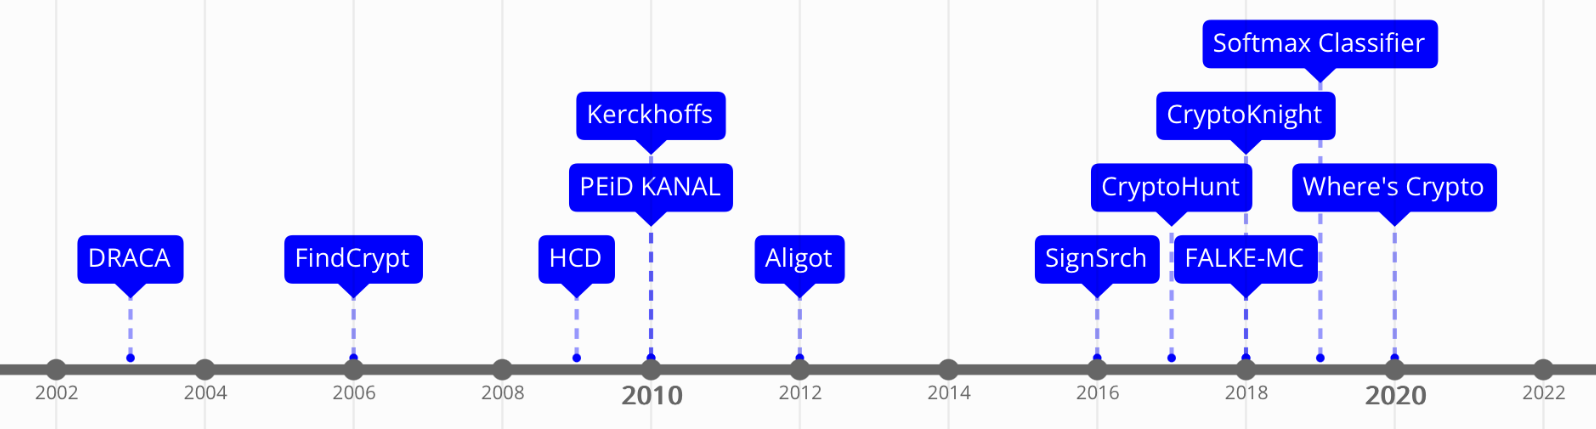
\includegraphics[width=0.95\textwidth,keepaspectratio]{ch-cryptobinary/figure/timeline.png}
  \caption{Timeline of the development of cryptographic algorithm detection tools}
  \label{fig:cryptobinary-tool_timeline}
\end{figure}

%%%%%%%%%%%%%%%%%%%%%%%%%%%%%%%%%%%%%%%%%%%%%%%%%%%%%%%%%%%%$$
\parhead{Cryptographic primitive vs. cryptographic function.} A brief note on notation used throughout this paper.  When we refer to a \textit{cryptographic function} or \textit{cryptographic algorithm}, we are generally referring to the entirety of a specific scheme or class of algorithms, such as RSA or hash functions.  When we say \textit{cryptographic primitive}, we generally mean a building block for a larger cryptographic scheme, such as a Feistel network.

%%%%%%%%%%%%%%%%%%%%%%%%%%%%%%%%%%%%%%%%%%%%%%%%%%%
\subsection{Categorization of Detection Approaches}
%%%%%%%%%%%%%%%%%%%%%%%%%%%%%%%%%%%%%%%%%%%%%%%%%%%
\label{sec:cryptobinary-detection}

Precision, scalability and performance of an identification approach all rely on the underlying techniques used.
Detection approaches can be divided into three categories:
i) Dynamic, ii) Static, and iii) Machine learning based approaches.

%%%%%%%%%%%%%%%%%%%%%%%%%%%%%%%%%

\parhead{Static Approaches.} Static approaches perform various forms of static analysis to detect
any static signatures, such as 'magic' constants, instruction sequences, and different code structures
such as S-boxes, as a means to identify cryptographic algorithms. This type of approach is based on the assumption that
cryptographic functions will perform a large number of arithmetic computations compared to non-cryptographic functions.
Harvey et al. \cite{harvey2001cipher} first proposed the idea of identifying cryptographic algorithms in binary files.
They focused on finding algorithms based on their constant
characteristics. By taking advantage of feature matching, subsequent
works \cite{lin2008automatic,caballero2007polyglot,wang2009reformat}
primarily focused on protocol reverse engineering. 
Chang et al. \cite{chang2014cryptographic} created a library of 3000 plus signature characteristics of cryptographic algorithms and also explored recognizing cryptographic algorithms based on Minimum Perfect Hash Function (MPHF).
Lestringant et al.~\cite{lestringant2015automated} used
data-flow isomorphism to find symmetric key algorithms.

Off-the-shelf tools such as Draft Crypto Analyzer
(DRACA)~\cite{draca}, Kanal~\cite{kanal}, Kerckhoffs~\cite{kerckhoffs},
Hash \& Crypto Detector (HCD)~\cite{hcd}, Signsrch~\cite{signsrch}, and Findcrypt~\cite{findcrypt2}, 
utilize static signature patterns of different cryptographic functions.
Static based approaches have low performance overhead. However, these
detection mechanisms can be easily bypassed using simple obfuscation techniques. For example,
the authors of Aligot~\cite{calvet2012aligot} showed that simple data obfuscation techniques
can bypass static analysis based detection mechanisms.

%%%%%%%%%%%%%%%%%%%%%%%%%%%%%%%%%%

\parhead{Dynamic Approaches.} Dynamic approaches~\cite{xu2017cryptographic,calvet2012aligot,li2012cipherxray}
primarily focus on identifying cryptographic primitives
from execution traces.
Lutz et al. \cite{lutz2008towards} first applied dynamic analysis to identify cryptographic algorithms based on three indicators:
i) presence of loops, ii) changes in entropy, and iii) high ratio of bitwise
arithmetic instructions.
Based on the data avalanche effect, CipherXRay~\cite{li2012cipherxray}
pinpoints the boundary of cryptographic operations and recovers transient
cryptographic secrets. However, this approach does not work in the case of stream
ciphers, for example, as they do not show any data avalanche effect.

Gr{\"o}bert et al.~\cite{grobert2011automated} proposed heuristic based 
approaches on both generic characteristics of cryptographic code and on
signatures for specific instances of cryptographic algorithms by mapping 
input-output (I/O) relations. Aligot~\cite{calvet2012aligot} further extends
this idea of I/O mapping. It retrieves
I/O parameters in an implementation-independent fashion, and compares
them with known cryptographic functions as well as performs
an interloop data flow analysis.
CryptoHunt~\cite{xu2017cryptographic} used bit-precise symbolic
loop mapping to identify cryptographic functions and applies guided fuzzing to
make the solution scalable. Park et al. \cite{park2020symmetric} proposed a hardware-assisted tracing technique to detect
symmetric-key cryptographic routines in anti-reverse engineered binaries via
recording the change of flow instructions from the CPU at run-time.
Dynamic approaches in general perform better than static based approaches in obfuscated
binaries, but suffer from much greater performance overhead.


%%%%%%%%%%%%%%%%%%%%%%%%%%%%%%%%%%%%%%%%%%%%%%%%% 

\parhead{Machine Learning Based Approaches.} With the growing popularity of machine learning, several recent works have explored utilizing such techniques.
Shin et al.~\cite{shin2015recognizing} discussed how recurrent neural networks can identify functions in binaries with greater accuracy and efficiency.
However, their approach was generalized for any function identification. 
For the purpose of cryptographic function identification,
Wright et al.~\cite{wright2009neural} proposed an artificial neural network model to classify
functional blocks as being either cryptographic or not by extracting the frequency of different logic instructions from a
disassembled program.
Benedetti et al. \cite{benedetti2017detection} used the `grap' tool to detect
cryptographic algorithms by creating patterns for AES and ChaCha20.
Falke~\cite{aigner2018falke} proposed a neural network based approach
by modeling classifiers for arbitrary cryptographic algorithms from
sample files and then automatically extracting features to train the neural
network. It offered a high detection rate in combination with
a low false positive rate.
Hill et al.~\cite{hill2018cryptoknight} proposed a Dynamic Convolutional Neural
Network based learning system (CryptoKnight) which learns from new cryptographic
execution patterns to classify unknown software.
Jia et al. \cite{jia2020neural} proposed an NLP-based approach which first extracts the
semantic information of assembly instructions and then transfers them into
100-dimensional vectors and later uses K-Max-CNN-Attention to classify
cryptographic functions.


%\parhead{Hybrid Solution.}
%\clg{This still needs to be filled out}


%\begin{figure}[h]
%	\includegraphics[width=\textwidth]{images/cryptoknight.pdf}
%	\caption{The CryptoKnight classification pipeline. 'Dynamic Binary Analysis' marked in red, is the point-of-failure.}
%\end{figure}


%The shared \texttt{CryptoTrace.so} object is built on the 32-bit \texttt{i386} architecture,
% and returns loading errors when run on \texttt{x86\_64} systems. 
 %On running the binary on an Ubuntu image running \texttt{i386}, d
 %ynamic instrumentation failed with segmentation faults, the stack trace displaying `\texttt{??? at CryptoTrace.so+0x7f550}' for every frame.


%\clg{This does not really seem relevant to the background section?  This seems like something that should maybe go in an appendix or something like that to explain why we couldn't test things?}

%\clg{I feel like background should maybe briefly introduce each tool, its techniques, and the algorithms it tries to target.  Or something like that.}
%\priyam{updated}


\subsection{Cryptographic Features}
\label{sec:cryptobinary-features}
%%%%%%%%%%%%%%%%%%%%%%%%%%%%%%%%
Cryptographic functions have their own (often quite distinct) set of characteristics, and work thus far has often leveraged these for identification, as they can lead to more tailored or performant techniques than general purpose binary analysis and code identification.
Many of these features only pertain to certain algorithms and cannot be used to identify others.
We now discuss some of the popular cryptographic features used for identification purposes.

%%%%%%%%%%%%%%%%%%%%%%%%%%%%
\parhead{Magic Constants.} In this approach, algorithm specific ``magic constants'' are searched for in the binary.  These are constant values that must occur in any implementation of a given algorithm.
%For example, the magic constants for the TEA algorithm usually are 2654435769 or
%0x9E3779B9. Existence of these constants in a binary can be used as a hint that it might contain TEA.
For instance, Signsrch~\cite{signsrch} relies on the magic number `0x9e3779b9' to detect the TEA algorithm; however, it fails to identify the algorithm when data obfuscation is applied~\cite{xu2017cryptographic}.

%%%%%%%%%%%%%%%%%%%%%%%%%%%%%%%%%
\parhead{Presence of Loops.} Most cryptographic functions use some form of loops for key generation, encryption, or other operations.
%For example, the factorization-based RSA algorithm has loops to perform modular exponentiation.
CryptoHunt~\cite{xu2017cryptographic} utilized loops as a means for detection. Given that loops may present in regular functions, further program analysis is necessary to ensure accurate detection.

%%%%%%%%%%%%%%%%%%%%%%%%%%%%%%%%%%
\parhead{Changes in Entropy.} The process of decryption usually decreases information entropy. Hence, entropy can be used as an indicator of  encrypted versus plaintext data. Several techniques~\cite{lutz2008towards, lee2022rcryptect} have used entropy to distinguish encrypted blocks from regular ones. 
However, relying on entropy can also lead to false positives in certain circumstances~\cite{grobert2011automated}.

%%%%%%%%%%%%%%%%%%%%%%%%%%%
\parhead{I/O Mapping.} Cryptographic functions sometimes have one-to-one mappings between their input to output, i.e., given a key and the plaintext, we might always get the same output, or given the input to a hash function, we should always get the same output. 
%These sort of unique one-to-one mappings can sometimes be used as indicators of the presence of cryptography (or even of specific deterministic algorithms like a hash function). 
However, these approaches rely on the accurate extraction of the key and input/output from the memory, as any wrong extraction can defeat the usefulness of unique mapping.
%data obfuscation
 
%%%%%%%%%%%%%%%%%%%%%%%%%%%%%%%%%%%%%
\parhead{Data-Flow Isomorphism.}
%A Data-Flow Graph (DFG) is a graph that represents data dependencies between a number of
%perations within a program~\cite{DFG}.
In this approach~\cite{lestringant2015automated}, a Data-Flow Graph (DFG)~\cite{DFG} is generated from the
corresponding assembly code, and subgraphs in the DFG are checked to see
whether they are isomorphic to the graph signature of a particular cryptographic
algorithm.
%This approach was first proposed by Lestringant
%et al~\cite{lestringant2015automated} and primarily used to identify symmetric
%key based algorithms. 
However, this approach is limited in the case of conditional
statements, which are more prominent in asymmetric algorithms. Additionally, DFG can
vary in effectiveness depending on data obfuscations techniques used in the implementation, such as data-splitting.

%%%%%%%%%%%%%%%%%%%%%
\parhead{S-Box.} Substitution boxes (S-Box)~\cite{sbox} are a fundamental component used in many symmetric key ciphers.
%An S-box is a table or function that swaps input bits with different bits, enhancing encryption security against attacks
%like differential and linear cryptanalysis, and often has a very distinct signature. 
For instance, the BLOWFISH algorithm
is a 64-bit block cipher that has an S-Box consisting of 1024 elements~\cite{jia2020neural} which are usually
sequentially stored in memory, allowing tools to detect BLOWFISH by locating this S-Box in memory. Similar techniques can be applied to Permutation Boxes (P-Box)~\cite{pbox}, which are methods of bit-shuffling to permute or transpose bits across S-box inputs.


%%%%%%%%%%%%%%%%%%%%%%%%%%%%%%%%%%%%
\parhead{Instruction Sequences.} An instruction sequence is a series of instructions or commands that a CPU executes in a specific order to perform tasks within a program. %These instructions can range from simple arithmetic calculations to more complex data manipulation and control flow operations. 
Many fundamental cryptographic operations will consist of fingerprintable instruction sequences and hence can be used for the purpose of identification. Nevertheless, this method may lose its effectiveness when dealing with control-flow obfuscations such as control-flow flattening~\cite{cfg_f}.




\subsection{Applications with Modern Cryptographic Algorithms}

Transport Layer Security (TLS) is a cryptographic protocol that is specifically crafted to facilitate secure communication over networks.

Starting from TLS 1.1, elliptic curve cryptography (ECC) has been incorporated into the TLS protocol. Furthermore, in TLS 1.3, ECC takes a central role in the base specification, featuring new signature algorithms, while RSA support has been discontinued. As of 2021, the deprecation of TLS 1.0 and 1.1 has taken place, resulting in ECC as the major choice for TLS ciphersuites.

There are numerous libraries that implement TLS, including OpenSSL, cryptlib, and Java Secure Socket Extension. Concurrently, beyond the TLS, a number of other applications leverage modern cryptographic algorithms. Notable examples include iMessage and Signal, both of which implement end-to-end encryption for enhanced security.


\section{Overview}
\label{sec:cryptobinary-overview}

This paper focuses on comprehensive replication and reproduction studies for existing work on identifying cryptography code in binary applications.
To aid in this, we propose a novel analysis framework aimed at facilitating a comprehensive evaluation of cryptographic function detection tools' replicability. Our framework is introduced in \autoref{sec:cryptobinary-framework}. Subsequently, we conduct two evaluations: a reproducibility evaluation in \autoref{sec:cryptobinary-reproduction}, and a replicability evaluation in \autoref{sec:cryptobinary-replication}. Additionally, we provide further discussion on the results of our reproducibility and replicability evaluations, as well as point out a number of important takeaways and directions for future work, in \autoref{sec:cryptobinary-discussion}. Finally, to support future research in this domain, we present a summary cryptographic detection approaches and tools in \autoref{sec:cryptobinary-background} as part of our background.

%%%%%%%%%%%%%%%%%%%%%%%

\subsection{Cryptographic Algorithm Detection Tools}

A number of cryptographic detection tools have been developed based on the different approaches discussed in \autoref{sec:cryptobinary-detection}. We perform our reproduction and replication studies on all existing work that we were able to find from 2000 until now:
\vspace*{-10pt}
\setlength{\columnsep}{-20pt}
\begin{multicols}{2}
\begin{itemize}[noitemsep,topsep=0pt]
    \setlength{\itemsep}{0pt}
    \setlength{\parskip}{0pt}
\item Aligot \cite{calvet2012aligot}
\item CryptoHunt \cite{xu2017cryptographic}
\item CryptoKnight \cite{hill2018cryptoknight}
\item DRACA \cite{draca}
\item FindCrypt2 \cite{findcrypt2}
\item FALKE-MC \cite{aigner2018falke}
\item HCD \cite{hcd}
\item Kerckhoff \cite{kerckhoffs}
\item PEiD KANAL \cite{kanal}
\item SignSrch \cite{signsrch}
\item Softmax Classifier \cite{jia2020neural}
\item Where's Crypto \cite{meijer2021s}
\end{itemize}
\end{multicols}
\vspace*{-5pt}
Our focus is on evaluating tools specifically designed for identifying cryptographic functions and comparing these tools with their stated performance. As such, we exclude other (broader) binary analysis tools, such as Binshape \cite{shirani2017binshape}, a general-purpose binary analysis tool, or CIS \cite{matenaar2012cis}, which focuses on testing cryptographic heuristics rather than actual algorithms.

We also employ a systematic approach to categorize, classify, and interrelate the diverse array of knowledge elements that constitute such tools from several directions in \autoref{subsec:cryptobinary-tool_cat}. We provide a more detailed discussion of each tool, along with its strengths and weaknesses, in \autoref{app:cryptobinary-tools}.

We comprehensively summarize the detection abilities of each cryptographic function detection tool. We did a thorough check of each tool's documents and signatures to see what types of cryptographic algorithms they can find. \autoref{fig:cryptobinary-percentage} shows the distribution of various algorithms that existing work has focused on.
After that, we gather all the information we found and explain it in more detail in \autoref{tab:cryptobinary-summary}. This helps us better understand what each tool can do in terms of detecting different cryptographic algorithms.

\begin{table*}[]
\centering
\setlength{\tabcolsep}{4pt}
\begin{adjustbox}{max width=\textwidth}
\renewcommand{\arraystretch}{1.5}
\begin{tabular}{l||c|c|c|c|c|c|c|c|c|c|c|c}
\hline
Tool & Aligot & \begin{tabular}[c]{@{}c@{}}Crypto-\\ Hunt\end{tabular} & \begin{tabular}[c]{@{}c@{}}Crypto-\\ Knight\end{tabular} & DRACA & FindCrypt2 & FALKE-MC & HCD & Kerckhoff & \begin{tabular}[c]{@{}c@{}}PEiD\\ KANAL\end{tabular} & SignSrch & \begin{tabular}[c]{@{}c@{}}Softmax\\ Classifier\end{tabular} & \begin{tabular}[c]{@{}c@{}}Where's\\ Crypto\end{tabular} \\ \hline\hline

ADLER32 &  &  &  &  &  &  & \multirow{35}{*}{\rotatebox[origin=c]{90}{\textit{Not Available}}} &  & \multirow{35}{*}{\rotatebox[origin=c]{90}{\textit{Not Available}}} &  & \cmark &  \\ \cline{1-7} \cline{9-9} \cline{11-13}
AES (Rijndael) & \cmark & \cmark & \cmark & \cmark & \cmark & \cmark &  & \cmark &  & \cmark &  & \cmark \\ \cline{1-7} \cline{9-9} \cline{11-13}
BASE64 &  &  &  &  &  &  &  &  &  & \cmark & \cmark &  \\ \cline{1-7} \cline{9-9} \cline{11-13}
Blowfish &  &  & \cmark & \cmark & \cmark &  &  &  &  & \cmark & \cmark &  \\ \cline{1-7} \cline{9-9} \cline{11-13}
Camellia &  &  &  &  & \cmark &  &  &  &  &  &  &  \\ \cline{1-7} \cline{9-9} \cline{11-13}
CAST &  &  &  &  & \cmark &  &  &  &  & \cmark &  &  \\ \cline{1-7} \cline{9-9} \cline{11-13}
CAST-256 &  &  &  & \cmark & \cmark &  &  &  &  & \cmark &  &  \\ \cline{1-7} \cline{9-9} \cline{11-13}
CRC32 &  &  &  & \cmark & \cmark &  &  &  &  & \cmark & \cmark &  \\ \cline{1-7} \cline{9-9} \cline{11-13}
DES &  &  &  & \cmark & \cmark &  &  & \cmark &  & \cmark & \cmark & \cmark \\ \cline{1-7} \cline{9-9} \cline{11-13}
EC &  &  &  &  &  &  &  &  &  & \cmark &  &  \\ \cline{1-7} \cline{9-9} \cline{11-13}
GOST &  &  &  &  & \cmark &  &  &  &  & \cmark &  &  \\ \cline{1-7} \cline{9-9} \cline{11-13}
HAVAL &  &  &  &  & \cmark &  &  &  &  & \cmark & \cmark &  \\ \cline{1-7} \cline{9-9} \cline{11-13}
MARS &  &  &  & \cmark & \cmark &  &  &  &  & \cmark &  &  \\ \cline{1-7} \cline{9-9} \cline{11-13}
MD2 &  &  &  &  & \cmark &  &  &  &  & \cmark &  &  \\ \cline{1-7} \cline{9-9} \cline{11-13}
MD4 &  &  &  &  & \cmark &  &  &  &  & \cmark &  &  \\ \cline{1-7} \cline{9-9} \cline{11-13}
MD5 & \cmark & \cmark & \cmark & \cmark & \cmark &  &  & \cmark &  & \cmark & \cmark & \cmark \\ \cline{1-7} \cline{9-9} \cline{11-13}
RC2 &  &  &  & \cmark & \cmark &  &  &  &  & \cmark &  &  \\ \cline{1-7} \cline{9-9} \cline{11-13}
RC4 & \cmark & \cmark & \cmark &  &  & \cmark &  & \cmark &  &  &  &  \\ \cline{1-7} \cline{9-9} \cline{11-13}
RC5 &  &  &  & \cmark & \cmark &  &  &  &  & \cmark & \cmark &  \\ \cline{1-7} \cline{9-9} \cline{11-13}
RC6 &  &  &  & \cmark & \cmark &  &  &  &  & \cmark & \cmark &  \\ \cline{1-7} \cline{9-9} \cline{11-13}
Ripemd-160 &  &  &  & \cmark &  &  &  &  &  & \cmark &  &  \\ \cline{1-7} \cline{9-9} \cline{11-13}
RSA & \cmark & \cmark & \cmark &  &  &  &  & \cmark &  &  &  &  \\ \cline{1-7} \cline{9-9} \cline{11-13}
SAFER &  &  &  & \cmark & \cmark &  &  &  &  & \cmark &  &  \\ \cline{1-7} \cline{9-9} \cline{11-13}
SHA-1 &  &  &  & \cmark & \cmark &  &  &  &  & \cmark & \cmark & \cmark \\ \cline{1-7} \cline{9-9} \cline{11-13}
SHA-256 &  &  &  &  & \cmark &  &  &  &  & \cmark & \cmark & \cmark \\ \cline{1-7} \cline{9-9} \cline{11-13}
SHA-512 &  &  &  &  & \cmark &  &  &  &  & \cmark &  & \cmark \\ \cline{1-7} \cline{9-9} \cline{11-13}
SHARK &  &  &  &  & \cmark &  &  &  &  & \cmark &  &  \\ \cline{1-7} \cline{9-9} \cline{11-13}
Skipjack &  &  &  & \cmark & \cmark &  &  &  &  & \cmark &  &  \\ \cline{1-7} \cline{9-9} \cline{11-13}
Square &  &  &  &  & \cmark &  &  &  &  & \cmark &  &  \\ \cline{1-7} \cline{9-9} \cline{11-13}
TEA & \cmark & \cmark &  & \cmark &  &  &  &  &  & \cmark &  &  \\ \cline{1-7} \cline{9-9} \cline{11-13}
Tiger &  &  &  & \cmark & \cmark &  &  &  &  & \cmark &  &  \\ \cline{1-7} \cline{9-9} \cline{11-13}
Twofish &  &  &  & \cmark & \cmark &  &  &  &  & \cmark &  &  \\ \cline{1-7} \cline{9-9} \cline{11-13}
WAKE &  &  &  &  & \cmark &  &  &  &  & \cmark &  &  \\ \cline{1-7} \cline{9-9} \cline{11-13}
Whirlpool &  &  &  &  & \cmark &  &  &  &  & \cmark &  &  \\ \cline{1-7} \cline{9-9} \cline{11-13}
XTEA &  &  &  &  &  &  &  &  &  &  &  & \cmark \\ \hline
\end{tabular}
\end{adjustbox}
%}
\caption{Cryptographic algorithm detection support as stated in the paper or documentation for each tool}
\label{tab:cryptobinary-summary}
\end{table*}

Note that we compiled these results based on information provided by the developers of each tool. Through our comprehensive analysis, we found that commercial tools like DRACA~\cite{draca}, FindCrypt2~\cite{findcrypt2}, and Signsrch~\cite{signsrch} can detect a diverse range of cryptographic algorithms. However, their performance falter when encountering obfuscation or atypical situations. Certain academic-developed tools such as Aligot~\cite{calvet2012aligot},  CryptoHunt~\cite{xu2017cryptographic}, and Where's Crypto~\cite{meijer2021s} offer superior analysis results in specific scenarios, such as detecting cryptographic algorithms from obfuscated binaries. Many of them can only detect a few cryptographic algorithm, but they can be easily expanded.

It is important to recognize that a simple summary may not fully capture the current capabilities and detection abilities of each tool. Moreover, many of these tools were developed years ago, and they may not be compatible with current programming languages, compilers, and/or hardware architectures.  This is why our reproduction and replication study is so crucial.  It not only highlights these major gaps in existing work as the space has progressed, but allows us to provide insights on the space more broadly, and on a variety of important avenues for future work.

\begin{figure}[t]
    \centering
    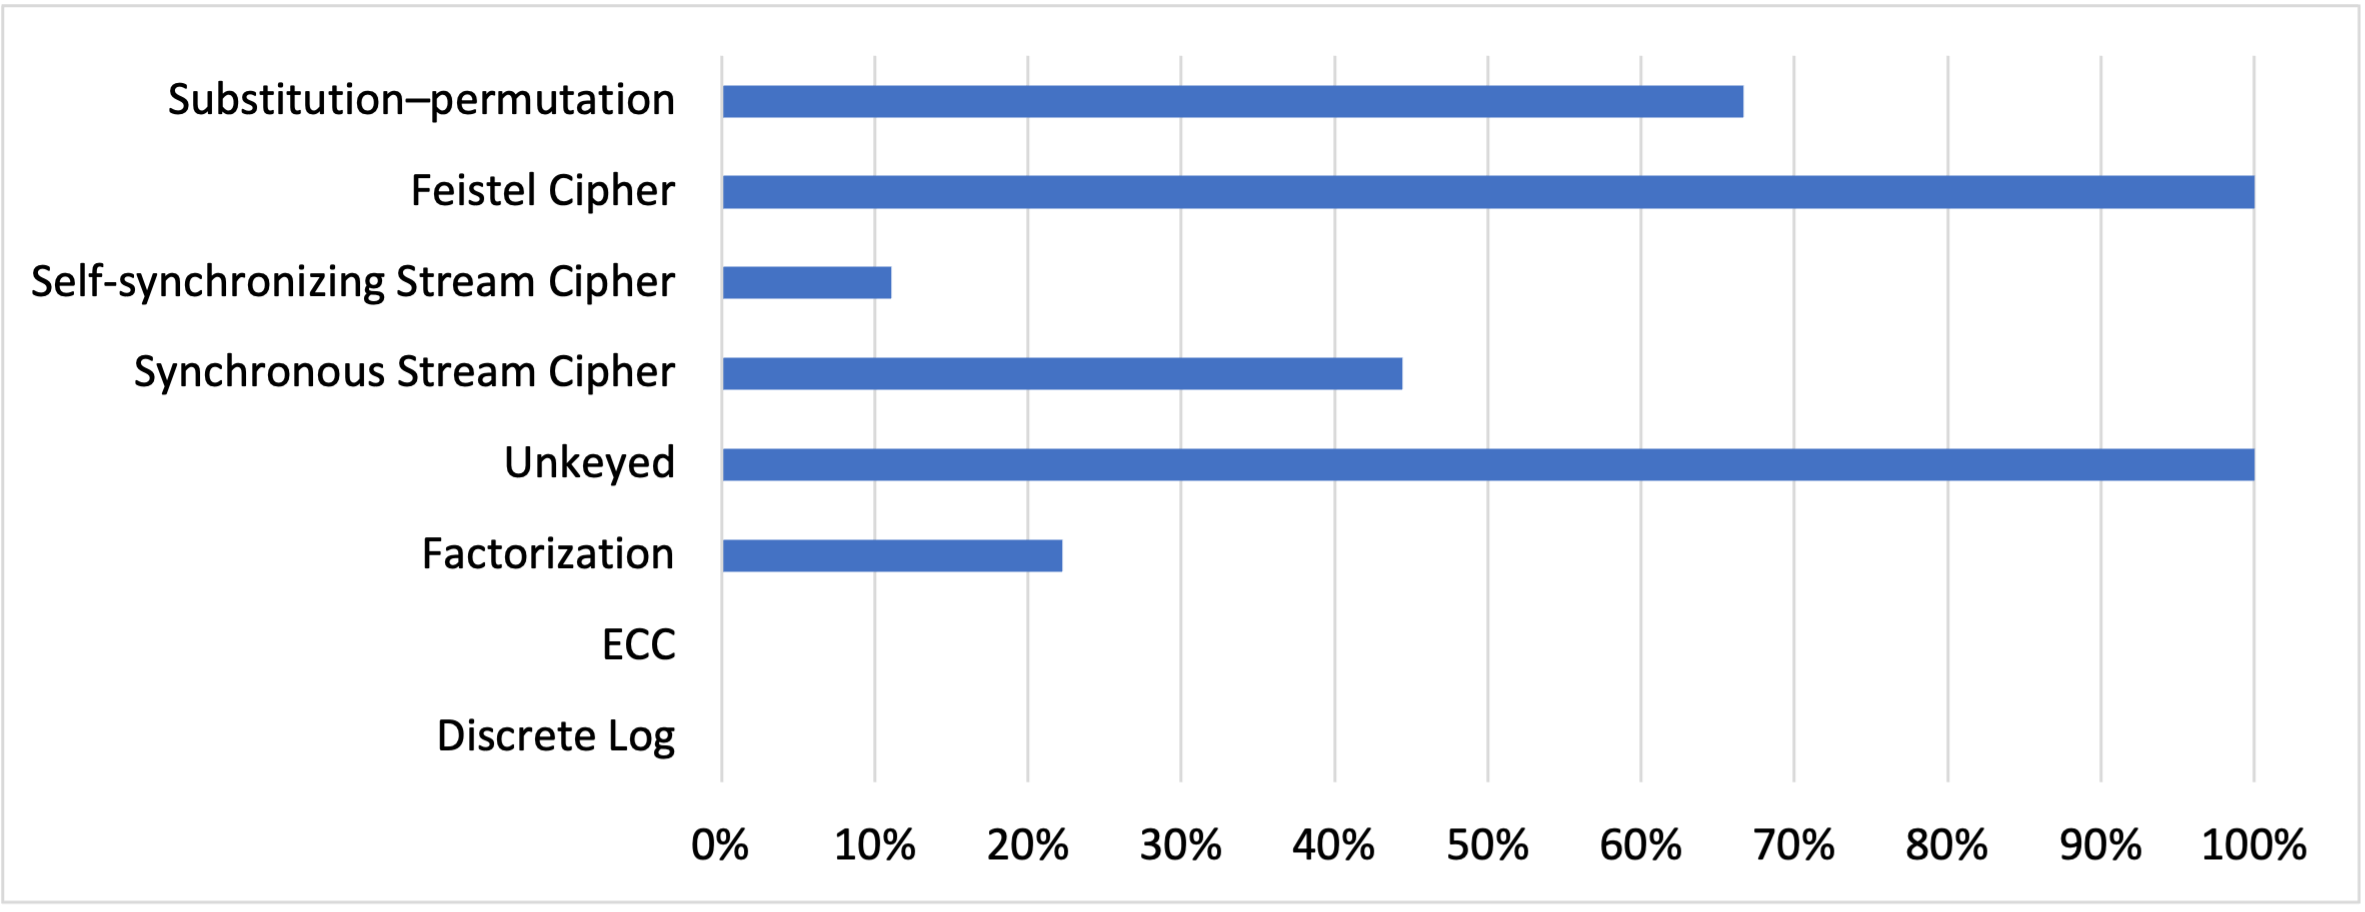
\includegraphics[width=0.95\textwidth]{ch-cryptobinary/figure/algo_percentage.png}
		\caption{Types of cryptographic functionality and designs targeted by different tools and approaches, by percentage of tools surveyed}
		\label{fig:cryptobinary-percentage}
\end{figure}

% \fanyo{To gain a comprehensive understanding of the current state of cryptographic function detection techniques and related tools, we conducted a comprehensive investigation experiment. We introduced numerous new evaluation benchmarks and frameworks that previous research in this field has not explored. Our benchmark will be detailed in Section \ref{sec:framework}, while the experiment results will be presented in Section \ref{sec:evaluation}. Additionally, we will provide discussion based on our evaluation results in Section \ref{sec:discussion}.}




% \fanyo{To gain a comprehensive understanding of the current state of cryptographic function detection techniques and related tools, we conducted a comprehensive investigation experiment. We introduced numerous new evaluation benchmarks and frameworks that previous research in this field has not explored. Our benchmark will be detailed in Section \ref{sec:framework}, while the experiment results will be presented in Section \ref{sec:evaluation}. Additionally, we will provide discussion based on our evaluation results in Section \ref{sec:discussion}.}






% %%%%%%%%%%%%%%%%%%%%%%%%%%%%%%%%%
% \subsection{Research Questions}
% %%%%%%%%%%%%%%%%%%%%%%%%%%%%%%%%%

% We also work to understand how well state-of-the-art techniques and tools perform by proposing and answering the following research questions.  We also believe many of these research questions are still yet unanswered in a satisfactory way, as we discuss more in Section~\ref{sec:evaluation} where we present a number of open research problems in these directions.

% \begin{itemize}
%   \item \textbf{R1} Does the choice of compiler play a role in the detection success? 
%   \item \textbf{R2} Is there any impact from optimization flags?
%   \item \textbf{R3} Are some algorithms easier to detect compared to others? 
%   \item \textbf{R4} Can the same tool perform similarly well across different algorithms?
%   \item \textbf{R5} Is the version of the algorithm significant during detection? 
%   \item \textbf{R6} Are ``malicious'' versions of cryptographic algorithms trickier to detect?

% \end{itemize}




\subsection{Categorization of Cryptographic Algorithm Detection Tools}
\label{subsec:cryptobinary-tool_cat}

We employ a systematic approach to categorize, classify, and interrelate the diverse array of knowledge elements that constitute such cryptographic detection tools from several directions. \autoref{tab:cryptobinary-taxonomy1} contains an overview and summary of each tool, including its reproduction and replication status in this work, as well as a variety of information such that one can easily find or organize existing (and future) tools based on the per-column categories.

We begin by categorizing the detection approach (broken down by the different methods discussed previously in ~\autoref{sec:cryptobinary-detection}) and the programming language in which the tool's source code is written. We note that some tools are not open source; they provide only an executable file, and as a result, we lack information about the source language.
Some tools require specific dependent libraries to run, which can limit or hinder their usability, and as such we list if there are any required dependencies.
Some tools are installation-free and do not require compilation, offering an easy, user-friendly experience.
And a few tools provide the capability for developers to insert new cryptographic algorithm signatures, thereby expanding their detection capabilities as the field advances.
 
\begin{sidewaystable}[p]
\centering
\footnotesize
\renewcommand{\arraystretch}{1.75}

\begin{adjustbox}{max width=0.9\textheight}
\begin{tabular}{c||c|c|c|c|c|c|c|c}
\hline
Tool & Method & \begin{tabular}{@{}c@{}}Dependent\\[-6pt]Library\end{tabular} & Language & \begin{tabular}{@{}c@{}}Requires\\[-6pt]Compiling\end{tabular} & Expandable & R+R & \begin{tabular}{@{}c@{}}Obf. Binary\\[-6pt]Design\end{tabular} & \begin{tabular}{@{}c@{}}AI/ML\\[-6pt]Approach\end{tabular} \\ \hline
\hline
Aligot         & I/O Parameters             & Intel Pin          & Python     & Yes     & Yes     & Reproducible & No  & No  \\ \hline
CryptoHunt     & Bit-precise Symbolic Loop  & Intel Pin          & C++        & Yes     & Yes     & Unable       & Yes & No  \\ \hline
CryptoKnight   & Machine Learning Based     & Intel Pin, PyTorch & Python     & Yes     & Yes     & Both         & No  & Yes \\ \hline
DRACA          & Unknown                    & None               & Executable & No      & No      & Replicable   & No  & No  \\ \hline
FindCrypt2     & Magic Constants            & IDA Pro            & C++        & Yes     & No      & Replicable   & No  & No  \\ \hline
FALKE-MC       & Neural Network             & None               & Unknown    & Unknown & Unknown & Unable       & Yes & Yes \\ \hline
HCD            & Unknown                    & None               & Executable & No      & No      & Replicable   & No  & No  \\ \hline
Kerckhoff      & Multiple                   & Intel Pin          & Python     & No      & Yes     & Unable       & No  & No  \\ \hline
PEiD KANAL     & Signature Searching        & None               & Executable & No      & Yes     & Replicable   & No  & No  \\ \hline
Signsrch       & Signature Searching        & None               & Executable & No      & No      & Replicable   & No  & No  \\ \hline
Softmax Classifier & Neural Network         & Unknown            & Python     & Unknown & Unknown & Unable       & No  & Yes \\ \hline
Where's Crypto & DFG Isomorphism            & IDA SDK            & C++        & Yes     & Yes     & Both         & No  & No  \\ \hline
\end{tabular}
\end{adjustbox}

\caption{Categorization of existing tools and their important properties}
\label{tab:cryptobinary-taxonomy1}
\end{sidewaystable}
\section{Analysis Framework for Open-Source Detection Tools}
%%%%%%%%%%%%%%%%%%%%%%%%%%%%%%%%%%%%%%%%%%%%%%%%%%%%%%%%%%%
\label{sec:cryptobinary-framework}

Previous tools have been evaluated only with certain basic cryptographic algorithms, and often seem to lack evaluation for false positives, real world applications, and large scale projects. Therefore, as the first step in our replication study, we build a new benchmarking framework with a number of evaluation metrics, which will not only encompass all evaluations conducted by previous tools but also establish a unified more comprehensive evaluation benchmark moving forward.

\fanyo{add transaction}

\vspace*{-10pt}
\begin{multicols}{3}
\begin{itemize}[noitemsep,topsep=0pt]
\item Aligot \cite{calvet2012aligot}
\item CryptoHunt \cite{xu2017cryptographic}
\item CryptoKnight \cite{hill2018cryptoknight}
\item DRACA \cite{draca}
\item FindCrypt2 \cite{findcrypt2}
\item HCD \cite{hcd}
\item PEiD KANAL \cite{kanal}
\item SignSrch \cite{signsrch}
\item Where's Crypto \cite{meijer2021s}
\end{itemize}
\end{multicols}
\vspace*{-10pt}

\subsection{Benchmarking Framework}
\label{subsec:cryptobinary-framework}
%%%%%%%%%%%%%%%%%%%
During our study, we identified a significant gap in the field: the absence of a standardized method for evaluating existing tools and their efficacy.
We believe that to do a fair evaluation in any domain requires a standard
benchmark. We propose a benchmarking framework that will help us understand the scalability
and effectiveness of any given detection approach. We have four categories in our framework: i) basic cryptographic functions, ii) microbenchmarks, iii) libraries, and iv) large projects.
Our framework is flexible and can be easily updated as the field of cryptography advances. 

\parhead{Basic cryptographic functions.} The basic cryptographic functions category contains cryptographic algorithms from various standard classes within the cryptographic space. A single cryptographic algorithm may have multiple versions, or may use non-standard implementations, so we may select many different implementations or versions for certain algorithms. The cryptographic algorithms we select are:

\vspace*{-10pt}
\begin{multicols}{3}
\begin{itemize}[noitemsep,topsep=0pt]
\item AES256
\item DES
\item ECC
\item MD5
\item RC4 
\item RC5
\item RSA
\item SHA1
\item SHA256
\item TEA
\item XTEA
\item XXTEA
\end{itemize}
\end{multicols}
\vspace*{-10pt}

We have chosen these algorithms for several reasons. First, we have included those recommended by the National Institute of Standards and Technology (NIST) \cite{nist}, as they are widely utilized and cover a broad range of real-world applications. Second, we have incorporated algorithms like TEA and MD5, which, although once popular, are now considered unsafe or outdated, but still might have historical significance in applications like malware. Last, we have selected various variants of a single cryptographic algorithm to assess a tool's ability to handle different implementations effectively.

\parhead{Microbenchmarks.} Our microbenchmarks category contains small programs on file
manipulation, networking, I/O heavy programs, math heavy programs, matrix and array, and so-called ``golden
implementations'' of well-known cryptographic algorithms. We have chosen small
programs such as I/O heavy and math-heavy programs since they have similar
instruction sets or behavior patterns as cryptographic functions.  This allows us to test for false positives in a detection framework.

\parhead{Libraries.} We have chosen cryptographic libraries as well as encoding and
compression libraries that have similar behavior to cryptographic
functions including:
\vspace*{-10pt}
\begin{multicols}{2}
\begin{itemize}[noitemsep,topsep=0pt]
\item openssl (3.3.1)
\item libgcrypt (1.8.11)
\item libsodium (1.0.20)
\item mbedTLS (3.6.1)
\item gnuTLS (3.8.6)
\item bzip2 (1.0.8)
\item zlib (1.3.1)
\item ffmpeg (7.0.2)
\item libgsm (1.0.17)
\item libjpeg (6b)
\item libpng (1.6.43)
\end{itemize}
\end{multicols}

This allows us to again test for false positives, but also to test for a variety of different cryptographic algorithms implemented in different ways.
We select open source libraries only, so that we are able to compile them based on our evaluation metrics. For each tool, we used the latest version available at the time of evaluation. Our selection includes a diverse range of libraries, from those with frequent recent updates, such as OpenSSL, to those that are a bit older, such as libjpeg.

\parhead{Large projects.} We also select Signal, an application designed for encrypted messaging, to evaluate a tool's ability to both scale for large codebases as well as still detect cryptography within them.  We believe that to understand the scalability of a mechanism, it is crucial to determine that the tool performs well irrespective of the code size and its applications.
Signal was selected because it both utilizes multiple (modern) cryptographic schemes and is open source.  This again means we can recompile Signal with our evaluation metrics, plus establish ground truth for testing. However, as our framework is open-source, one could easily extend it to include any future desired large-scale open-source projects, such as Tor.

\subsection{Evaluation Metrics}
\label{subsec:cryptobinary-metrics}
To ensure a thorough exploration of current tools (and to provide rigorous and fair evaluation metrics for the future), we have meticulously crafted a series of evaluation experiments. These experiments are thoughtfully designed to align with the challenges we discuss in \autoref{subsec:cryptobinary-challenges}, maximizing our ability to uncover the current state of these tools and elucidate their strengths and weaknesses.  Our evaluation metrics are as follows:
 
\begin{itemize}
\item \textbf{Based on optimization levels:} Evaluate based on different compiler optimizations including \texttt{-O0}, \texttt{-O1}, \texttt{-O2}, \texttt{-O3}, \texttt{-Os}, and \texttt{-Ofast}.

\item \textbf{Based on different combinations of obfuscation mechanisms:}

\begin{itemize}
\item \textbf{Control-flow obfuscation:} Adding bogus control-flow, control-flow flattening, substitution of instructions, polymorphism.

\item \textbf{Data-flow obfuscation:} Data aggregation, data-splitting, variable transformation.

\item \textbf{Modified versions of algorithms:} For example, modified TEA (Russian TEA) used in malware as suggested in \cite{xu2017cryptographic}.

\item \textbf{Layout Obfuscation:} Address obfuscation, obfuscating debug information, address layout/memory layout randomization .

\item \textbf{Combination of prior techniques}
\end{itemize}
% \item \textbf{Based on type of the algorithm:} Some approaches can work better on stream ciphers, some others can work better on block ciphers

\item \textbf{Based on different compilers:} Evaluate based on different compilers, including GCC, CLANG, MSVC.
% \item \textbf{Based on algorithm versions:} A single cryptograhic algorithm may have multiple variant versions, and some malware do not use standard algorithm implementation.

\end{itemize}

The full list of optimizations, obfuscations, and their combinations selected for our evaluation is shown below.

\begin{enumerate}
\setcounter{enumi}{-1}
\item No identification
\item Identification with optimization flag \texttt{-O0}
\item Identification with optimization  flag \texttt{-O1}
\item Identification with optimization flag \texttt{-O2}
\item Identification with optimization flag \texttt{-O3}
\item Identification with optimization flag \texttt{-Os}
\item Identification with optimization flag: \texttt{-Ofast}
\item Identification with instruction substitution obfuscation: \texttt{-obs\textunderscore sub}
\item Identification with control-flow flattening: \texttt{-obs\textunderscore fla}
\item Identification with bogus control-flow: \texttt{-obs\textunderscore bcf}
\item Identification with combination of obfuscation: \texttt{-obs\textunderscore sub}, \texttt{-obs\textunderscore fla}, \texttt{-obs\textunderscore bcf}
\item Identification with combination of obfuscation and optimization: \texttt{-obs\textunderscore sub}, \texttt{-obs\textunderscore fla}, \texttt{-obs\textunderscore bcf}, \texttt{-O3}
\end{enumerate}

%\section{Identiifcation techniques}
%%%%%%%%%%%%%%%%%%%%%%%%%%%%%%%%%%%


%%%%%%%%%%%%%%%%%%%%%%%%%%%%%%%
%\begin{figure}[ht]
%\centering{
%  \subfigure[Evaluation of DRACA based on performance metrics]{%
%    \includegraphics[width=\columnwidth, keepaspectratio]{./images/draca.pdf}
%    \label{fig:draca}}
%  \subfigure[Evaluation of Signsrch based on performance metrics]{%
%    \includegraphics[width=\columnwidth, keepaspectratio]{./images/signsrch.pdf}
%    \label{fig:signsrch}}
%    %\caption{}
%}
%\end{figure}

% \begin{figure}[ht]
% \centering
% \begin{minipage}{.45\textwidth}
%   \centering
%   \includegraphics[width=\linewidth]{./images/draca.pdf}
%   \caption{Evaluation of DRACA based on performance metrics}
%   \label{fig:draca}
% \end{minipage}%
% \qquad
% \begin{minipage}{.45\textwidth}
%   \centering
%   \includegraphics[width=\linewidth]{./images/signsrch.pdf}
%   \caption{Evaluation of Signsrch based on performance metrics}
%   \label{fig:signsrch}
% \end{minipage}
% \end{figure}

We assessed each tool with these benchmarks and metrics to thoroughly explore accuracy and detection capabilities when handling binary programs subjected to specific compiler or optimization/obfuscation techniques.\footnote{All benchmarks and metrics we evaluate are available at \url{https://github.com/BARC-Purdue/CryptoBinary}.} For instance, a tool \textbf{A} might successfully detect MD5 when all optimization flags are applied but fail to do so in the presence of obfuscation. Conversely, a tool \textbf{B} may be able to detect TEA when compiled with GCC but not when compiled with CLANG. This exploration provides us with a more comprehensive understanding of the current state of cryptographic function detection tools, revealing their weaknesses and indicating areas for future development from various perspectives.


% Then based on our metric, we give tool \textbf{A}
% score of 7 in unkeyed category. \autoref{fig:draca} and \autoref{fig:signsrch}
% shows the performance of the two tools namely DRACA and Signsrch based on
% the above mentioned metrics.





% \subsection{A Benchmark Framework}
% % For large scale project, we have chosen signal given its large code base and
% % wide spread usage. \autoref{benchmarks} shows the analysis of two tools DRACA
% % and signsrch across all the three categories of the benchmarks as well as with
% % different compilation and obfuscation flags.

% We categorized our framework in couple of directions. We can categorize them based on size to understand the scalability of each of the investigated tools. Then, we can categorize based on the type of the suite. Here are four possible categorizations: 

% \textbf{i. In accordance to size:} We can evaluate different types of projects based on size to understand  the effectiveness of tool 

% a. Micro-benchmarks  

% b. Small/ medium sized projects

% c. Large projects

% \textbf{ii. In accordance to type:} We can develop a number of test-suites which shows crypto like behavior. Possible options are: network-heavy test-suite, mathematics-heavy suite, binary packing, suite with extraction operations.

% \textbf{iii. Real world open-source projects:} We can select a good number of real world open source projects to understand the effectiveness of investigated tools.

% \textbf{iv. Real malware samples:} Possible malware: wannacry (Windows encryption API), petya, not-petya, locky (RSA-2048 + AES-128 cipher with ECB mode), Annabele (AES256 CBC with a hardcoded key and IV). Petya and NotPetya both read the MBR and encrypt it using a simple XOR key. The only difference is that Petya uses 0x37 as a key, while NotPetya uses 0x07.


%algorithm vs functionalities 


\section{Reproduction}
\label{sec:cryptobinary-reproduction}
% To verify the reproducibility and replicability for each tool, we conduct a end-to-end evaluation experiment as the following procedure
% \begin{itemize}
%   \item Compile the tool's source code from sketch in different operating system (Windows, Mac OS, and Linux) if source code is provided
%   \item Evaluate the benchmark provided by original tool if provided.
%   \item Evaluate each tool with our new  benchmark system
% \end{itemize}

We start by assessing the reproducibility of each tool by employing consistent experimental setups, procedures, and operating conditions to replicate their purported capabilities. 

In our reproducibility evaluation we follow the ACM guidelines on reproducibility \cite{rar}, using the same measurement procedure, system setting, and operating conditions as the tool's original test cases\footnote{For the precise details and steps of our reproducibility evaluation see Appendix \ref{app:cryptobinary-repro_procedure}.}. This will help us to understand the basic fundamental reliability for each tool.  When tools do not pass the reproduction evaluation, we also provide a brief discussion for why.
\autoref{tab:cryptobinary-reproducibility} shows the reproducibility results.
% \fanyo{We use \cmark to indicate successful reproduction of the tool with their original test cases, \xmark for failure to reproduce or when the tool is unavailable (neither source code nor compiled binary is provided), and \texttt{n/a} if the tool is executable but lacks the original test cases.}

\begin{table}[h]
\centering
\begin{adjustbox}{max width=\textwidth}
\begin{tabular}{c|c|c|c|c|c}
\hline
Aligot & \makecell{Crypto\\Hunt} & \makecell{Crypto\\Knight}  & DRACA  & FindCrypt2  & FALKE-MC \\ \hline
\cmark & \xmark & \cmark & \textminus & \textminus & \xmark  \\ \hline \hline
HCD & Kerckhoff  & \makecell{PEiD \\ KANAL}  & SignSrch  & \makecell{Softmax \\ Classifier}  & \makecell{Where’s \\ Crypto}\\ \hline
\textminus  & \xmark & \textminus & \textminus & \xmark & \cmark  \\ \hline
\end{tabular}
\end{adjustbox}
\caption{Reproducibility outcome for each tools. \cmark~indicates a tool that has passed the reproduction evaluation, while \xmark~represents a tool that has either failed the reproduction evaluation or is not accessible. \textminus~denotes a tool that is available for use, but the developer has not provided the original test cases.}
\label{tab:cryptobinary-reproducibility}
\vspace{-10pt}
\end{table}

Note that for certain tools, the developers only provided the executable binary program without the accompanying source code or test cases necessary for evaluation, making a reproducibility assessment unfeasible (denoted \textminus). Some tools are not publicly available in either source code or executable binary form, making a reproducibility evaluation impossible. As a result, they are marked with a \xmark. Additionally, we encountered crashes when running Pin-based tools with the latest version of Intel Pin, indicating that the design of older cryptographic detection tools may not be compatible with newer Pin versions. However, Aligot is the one exception to this.  Aligot provides step-by-step test cases, and, based on this, we have successfully reproduced each step with the expected results. Therefore, we consider Aligot reproducible, as we were able to replicate the test results using their original measurement procedures.

\subsection{Non-Reproducible Tools}
\parhead{CryptoHunt} has been successfully executed, but we are unable to provide the complete benchmarking framework and performance evaluation results. CryptoHunt detects cryptographic functions in binary code through a bit-precise symbolic loop mapping approach. However, depending on the binary's size, CryptoHunt may identify up to 10,000 loops within the binary. Without additional filtering, the process of comparing each of these loops with reference loops becomes exceedingly time-consuming and infeasible.

\parhead{Kerckhoff} cannot be evaluated in this paper due to its incompatibility with existing available versions of the Pin tracing tool, which cause it to crash. We have encountered a similar issue in the replication evaluation as well, which will be discussed in \autoref{sec:cryptobinary-replication}.
%This issue may be similar to the experience we have with Aligot, which informs future researchers that detection tools developed to depend on specific tracing functionalities may not age well or be suitable for current/future binary programs. \clg{Also not sure what you mean here with Aligot since that one worked? Also check what I rephrased here.}

\parhead{Softmax Classifier \textnormal{and} FALKE-MC} cannot be evaluated in this paper since they are not available for public use, as neither the source code nor the compiled binary is provided. Only the original research paper is available, with no accompanying software or executable.

\section{Replication}
\label{sec:cryptobinary-replication}

We now undertake a comprehensive replicability evaluation of existing work across different categories of cryptographic algorithms with our newly proposed analysis framework, in order to understand their consistency, robustness, and effectiveness. Our replication evaluation follows the ACM guidelines on replicability \cite{rar}. We rebuild each tool (if the source code is available) and run it across different system environments using our newly developed evaluation benchmark as the test cases\footnote{For the precise details and steps of our replicability evaluation see Appendix \ref{app:cryptobinary-repli_procedure}.}.
This evaluation encompasses all work across this domain, allowing us to delve into their performance and potential limitations. For each cryptographic algorithm, we considered different optimization/obfuscation levels, compilers, and implementations. These experiments are designed to help us understand the consistency and robustness of existing work and techniques, the current status of cryptographic function detection performance and to explore potential future research questions, as well as to highlight existing challenges in cryptographic function detection.  We also involve micro-benchmarks, libraries, and large scale projects to examine each tool's performance in real-world applications.
We present the full results of our evaluation in Table~\ref{tab:cryptobinary-benchmarks} in Appendix~\ref{app:cryptobinary-addltables}, and discuss a selection of the results, as well as their implications, now.

Based on our replicability evaluation, we find that some tools cannot be replicated with our framework. We also highlight some interesting new results, which may help direct future research in this field. This will be addressed in both this section and in Section \ref{sec:cryptobinary-discussion}.


\subsection{Non-Replicable Tools}

\parhead{Aligot} is a cryptographic function identification tool developed based on Pin, a dynamic binary instrumentation framework developed by Intel. We successfully reproduce the test cases that Aligot provided. However, Aligot was tested with Pin 2.10 and Pin 2.12 by its developer, but unfortunately, these versions are no longer available. Consequently, we attempted to use an older version of Pin (3.22) but we were unable to execute Aligot correctly. We believe this to be due to the fact that this tool does not support and cannot be executed on recent CPU architectures.



% \begin{table}[]
% \footnotesize
% \centering
% \begin{tabular}{|cl||c|c|c|c|c|c|c|}
% \hline
% \multicolumn{2}{|c||}{Tool} & \rotatebox[origin=c]{90}{CryptoKnight} & \rotatebox[origin=c]{90}{DRACA} & \rotatebox[origin=c]{90}{Findcrypt2} & \rotatebox[origin=c]{90}{HCD} & \rotatebox[origin=c]{90}{PEiD KANAL} & \rotatebox[origin=c]{90}{SignSrch} & \rotatebox[origin=c]{90}{Where's Crypto} \\ \hline\hline
% \multicolumn{1}{|l|}{\multirow{8}{*}{Algorithm}} & AES & {\color{green}\CIRCLE} & {\color{red}\warn} & {\color{red}\warn} &  &  & {\color{green}\CIRCLE} & {\color{green}\CIRCLE} \\ \cline{2-9} 
% \multicolumn{1}{|l|}{} & DES &  & {\color{red}\warn} & {\color{green}\CIRCLE} &  &  & {\color{red}\warn} & {\color{green}\CIRCLE} \\ \cline{2-9} 
% \multicolumn{1}{|l|}{} & MD5 & {\color{red}\warn} & {\color{green}\CIRCLE} & {\color{green}\CIRCLE} &  &  & {\color{green}\CIRCLE} & {\color{green}\CIRCLE} \\ \cline{2-9} 
% \multicolumn{1}{|l|}{} & RC4 & {\color{red}\warn} &  &  &  &  &  &  \\ \cline{2-9} 
% \multicolumn{1}{|l|}{} & RC5 &  & {\color{green}\CIRCLE} & {\color{green}\CIRCLE} &  &  & {\color{green}\CIRCLE} &  \\ \cline{2-9} 
% \multicolumn{1}{|l|}{} & RSA & {\color{green}\CIRCLE} &  &  &  &  &  &  \\ \cline{2-9}
% \multicolumn{1}{|l|}{} & SHA-1 &  & {\color{green}\CIRCLE} & {\color{green}\CIRCLE} &  &  & {\color{green}\CIRCLE} & {\color{green}\CIRCLE} \\ \cline{2-9} 
% \multicolumn{1}{|l|}{} & SHA-256 &  &  & {\color{green}\CIRCLE} &  &  & {\color{green}\CIRCLE} & {\color{green}\CIRCLE} \\ \cline{2-9} 
% \multicolumn{1}{|l|}{} & TEA &  & {\color{green}\CIRCLE} &  &  &  & {\color{green}\CIRCLE} & {\color{green}\CIRCLE} \\ \hline

% \end{tabular}
% \caption{Comparison}
% \label{tab:comparison}
% \end{table}



% \begin{table}[]
% \begin{tabular}{|l|lllllllll|}
% \hline
% \multirow{2}{*}{Tool} & \multicolumn{9}{l|}{Algorithm} \\ \cline{2-10} 
%  & \multicolumn{1}{l|}{TEA} & \multicolumn{1}{l|}{RC4} & \multicolumn{1}{l|}{RC5} & \multicolumn{1}{l|}{DES} & \multicolumn{1}{l|}{AES} & \multicolumn{1}{l|}{SHA-1} & \multicolumn{1}{l|}{SHA-256} & \multicolumn{1}{l|}{MD5} & RSA \\ \hline
% DRACA & \multicolumn{1}{l|}{{\color{green}\cmark}} & \multicolumn{1}{l|}{} & \multicolumn{1}{l|}{{\color{green}\cmark}} & \multicolumn{1}{l|}{{\color{red}\warn}} & \multicolumn{1}{l|}{{\color{green}\cmark}} & \multicolumn{1}{l|}{{\color{green}\cmark}} & \multicolumn{1}{l|}{} & \multicolumn{1}{l|}{{\color{green}\cmark}} &  \\ \hline
% Findcrypt2 & \multicolumn{1}{l|}{} & \multicolumn{1}{l|}{} & \multicolumn{1}{l|}{{\color{green}\cmark}} & \multicolumn{1}{l|}{{\color{green}\cmark}} & \multicolumn{1}{l|}{{\color{red}\warn}} & \multicolumn{1}{l|}{{\color{green}\cmark}} & \multicolumn{1}{l|}{{\color{green}\cmark}} & \multicolumn{1}{l|}{{\color{green}\cmark}} &  \\ \hline
% HCD & \multicolumn{1}{l|}{} & \multicolumn{1}{l|}{} & \multicolumn{1}{l|}{} & \multicolumn{1}{l|}{} & \multicolumn{1}{l|}{} & \multicolumn{1}{l|}{} & \multicolumn{1}{l|}{} & \multicolumn{1}{l|}{} &  \\ \hline
% PEiD KANAL & \multicolumn{1}{l|}{} & \multicolumn{1}{l|}{} & \multicolumn{1}{l|}{} & \multicolumn{1}{l|}{} & \multicolumn{1}{l|}{} & \multicolumn{1}{l|}{} & \multicolumn{1}{l|}{} & \multicolumn{1}{l|}{} &  \\ \hline
% SignSrch & \multicolumn{1}{l|}{{\color{green}\cmark}} & \multicolumn{1}{l|}{} & \multicolumn{1}{l|}{{\color{green}\cmark}} & \multicolumn{1}{l|}{{\color{red}\warn}} & \multicolumn{1}{l|}{{\color{red}\warn}} & \multicolumn{1}{l|}{{\color{green}\cmark}} & \multicolumn{1}{l|}{{\color{green}\cmark}} & \multicolumn{1}{l|}{{\color{red}\warn}} &  \\ \hline
% CryptoKnight & \multicolumn{1}{l|}{} & \multicolumn{1}{l|}{{\color{red}\warn}} & \multicolumn{1}{l|}{} & \multicolumn{1}{l|}{} & \multicolumn{1}{l|}{{\color{green}\cmark}} & \multicolumn{1}{l|}{} & \multicolumn{1}{l|}{} & \multicolumn{1}{l|}{{\color{red}\warn}} & {\color{green}\cmark} \\ \hline
% Where's Crypto & \multicolumn{1}{l|}{{\color{green}\cmark}} & \multicolumn{1}{l|}{} & \multicolumn{1}{l|}{} & \multicolumn{1}{l|}{{\color{green}\cmark}} & \multicolumn{1}{l|}{{\color{green}\cmark}} & \multicolumn{1}{l|}{{\color{green}\cmark}} & \multicolumn{1}{l|}{{\color{green}\cmark}} & \multicolumn{1}{l|}{{\color{green}\cmark}} &  \\ \hline
% \end{tabular}
% \label{tab:comparison}
% \caption{Comparison}
% \end{table}



% \subsection{Benchmark Evaluation}
% We firstly evaluate these tool with cryptographic function in our new developed benchmark. We do find some previous evaluate result that cannot be reproduce, which has been introduce in \autoref{subsec:unreproduce}

% In our micro-benchmark evaluation, we also find some false positive result. None of the tool falsely consider file handle, I/O, network connection, or heave math operation as cryptographic function. However, CryptoKnight and Signsrch miss claim a mathematical matrix as cryptographic function such as AES. AES algorithm has Rijndael S-box, so cryptographic function detection tool with static signature search approach may false reconazation a matrix as AES function.

% Finally, besides the standard cryptographic function, we also select some crypthrapgic. We find that many tool detect cryptographic function from these libraries since some of these libraries such as openssl and libgcrypt do have cryptographic function in the binary. However, some tool cannot correctly detect cryptographic function in real world applications 
% For example, DRACA, HCD, and Signsrch cannot detect any cryptographic function from openssl; CryptoKnight and HCD cannot detect cryptographic function from libgcrypt etc.

\subsection{Unexpected Detection Results}
\label{subsec:cryptobinary-false}

\begin{table}[]
\footnotesize
\centering
\begin{adjustbox}{max width=\textwidth}
\begin{tabular}{c||c|c|c|c|c|c|c|c|c}
\hline
\multirow{2}{*}{Tool} & \multicolumn{9}{c}{Cryptographic Algorithm} \\ \cline{2-10}
& AES & DES & MD5 & RC4 & RC5 & RSA & SHA1 & SHA256 & TEA \\ \hline
\hline
DRACA & \xmark & \xmark & \cmark &  & \cmark &  & \cmark &  & \cmark \\ \hline
CryptoKnight & \cmark &  & \xmark & \xmark &  & \cmark &  &  &  \\ \hline
FindCrypt2 & \xmark & \cmark & \cmark &  & \cmark &  & \cmark & \cmark & \cmark \\ \hline
HCD         & \textminus & \textminus & \textminus & \textminus & \textminus & \textminus & \textminus & \textminus & \textminus \\ \hline
PEiD KANAL & \textminus & \textminus & \textminus & \textminus & \textminus & \textminus & \textminus & \textminus & \textminus \\ \hline
SignSrch & \cmark & \xmark & \cmark &  & \cmark &  & \cmark & \cmark & \cmark \\ \hline
Where's Crypto & \cmark & \cmark & \cmark &  &  &  & \cmark & \cmark & \cmark \\ \hline
\end{tabular}
\end{adjustbox}
\caption{Comparative analysis of detection approaches versus stated capabilities in original documentation. Cross mark denotes inconsistencies (false positive or false negative), check mark successful replication.}
\label{tab:cryptobinary-comparison}
%\vspace{-20pt}
\end{table}

We begin by discussing evaluation results that were either unexpected or inconsistent based on prior stated findings.
During our evaluation, we encountered instances where certain tools yielded false positives or false negatives in their detection outcomes. These findings underline the importance of a more in-depth and rigorous analysis to ensure the attainment of dependable detection results. As a result, it is evident that further development is required to enhance reliability.

\parhead{Unreplicable cryptographic function detection.} In \autoref{tab:cryptobinary-summary}, we list the purported performance for each tool. However, our evaluation could not verify the detection capabilities for certain cryptographic functions in some of the tools. \autoref{tab:cryptobinary-comparison} presents the outcomes of our assessment relative to the detection capabilities as claimed by the respective tools' original documentation. If a tool claims to have the ability to detect a cryptographic algorithm, but we cannot reproduce the same result in any of our benchmarks or evaluation metrics, we mark it with a red exclamation mark. Otherwise, if we can confirm the detection ability, we mark it with a green circle. A blank means the tool makes no claim about the given algorithm.  Due to the unavailability of documentation for HCD and PEiD KANAL, a comparison of our evaluation results with their claimed detection capabilities was not possible.

\parhead{Micro-benchmark false positives.} In our micro-benchmark evaluations, we also uncovered new false positive results. None of the tools falsely considered operations like file handling, I/O, network connection, or heavy math operations as cryptographic functions. However, some tools, such as CryptoKnight and Signsrch, mistakenly identify a mathematical matrix as a cryptographic function like AES. Since AES includes the Rijndael S-box (often coded as a matrix), tools that rely on static signature searches may incorrectly recognize a matrix as an AES function. This highlights the importance of broader and more standardized test cases as well, as things like this were not considered by previous evaluations.
To better understand these results, in Table \ref{tab:cryptobinary-quat} (Appendix~\ref{app:cryptobinary-addltables}) we present the detailed breakdown of percentage of false positives and false negatives observed for each tool across various cryptographic functions, offering a comprehensive comparison of their performance in these error metrics. This allows us to gain insight into the likelihood of a tool raising errors when attempting to detect specific cryptographic functions.

\parhead{Undetected cryptographic functions in libraries.} Finally, besides standard stand-alone cryptographic functions, we also selected some real-world cryptographic libraries and libraries with similar behavior to cryptographic functions to test on. We find that many tools successfully detect cryptographic functions in these libraries, which is expected, as some, including openssl and libgcrypt, are indeed primarily cryptographic libraries.
However, it is interesting to note that this is not true of all tools.  Some work fails to detect cryptographic functions in this setting.  For example, tools like DRACA, HCD, and Signsrch are unable to detect any cryptographic functions from openssl, while CryptoKnight and HCD fail to detect cryptographic functions in libgcrypt. We are not sure why this is the case, and leave this as an interesting avenue for future work.  This also points to the fact that existing work may have unreliable performance in real world (large) programs.

\begin{takeaway}
\textbf{Future Research:} Certain cryptographic-specific libraries seem to pose challenges for existing tools; exploring why this is the case would be an interesting avenue for future work.  Also, existing tools have more false positives/negatives than initially expected, so placing more emphasis on improving detection accuracy and reducing false positives or false negatives seems highly relevant.
\end{takeaway}

% For example, when we carried out our evaluations on a binary that contained RC5, we observed that DRACA, Signsrch, and HCD effectively detected the presence of the RC5 function. However, it is noteworthy that they also identified the TEA function. Both TEA and RC5 belong to the block cipher family, which occasionally leads to the occurrence of false positives and noise in function detection. This situation underscores the importance of exercising caution when a tool identifies multiple cryptographic functions within the same category, as such detections could potentially be false positives resulting from the analysis approaches or weaknesses of the tool itself.

% We also observed instances where certain tools produced false negatives. Some tools claimed to have the capability to detect specific algorithms, but we were unable to reproduce these results. Based on the full evaluation results in Table \ref{tab:benchmarks}, it is evident that AES and DES cannot be detected by many tools, even though many of them should theoretically have the ability to do so.

\subsection{Operating System Limitations}

The usage of certain tools may be constrained by their exclusive compatibility with specific operating systems, impacting their efficacy and analysis capabilities. Many tools are designed and built with specific operating systems in mind.  Fortunately, with the help of other tools, such as WineHQ, which enables software developed for Microsoft Windows to run on Unix-like operating systems, developers can for example use some Windows cryptographic detection tools in Linux. However, tools are not just limited to running on specific operating systems, but also restricted to handling binaries compiled for selected operating systems.
These inherent limitations potentially reduce the scope and depth of analysis a tool can provide, depending on the operating system selected and targeted in the original work.

%For example, most malware is designed for a specific operating system. In order to detect malware and its related cryptographic functions, a developer has to use a cryptographic detection tool that supports the target operating system, or otherwise, such analysis will be hampered.

In Table \ref{tab:cryptobinary-system}, we evaluate the capability of exisiting work to analyze binaries across three different operating systems and for binaries compiled specifically for each of these operating systems. We use a \LEFTcircle \space to indicate cases where a tool cannot be executed on a Unix-like system but becomes functional with the assistance of WineHQ.

\begin{takeaway}
\textbf{Takeaway:} Ideally cryptographic function detection tools need to support all operating systems to effectively detect cryptographic functions or malware across diverse environments and improve overall detection measures.
\end{takeaway}

% Please add the following required packages to your document preamble:
% \usepackage{multirow}
%\vspace*{-10pt}
\begin{table}[t]
\centering
\begin{adjustbox}{max width=\textwidth}
\begin{tabular}{c||ccc||ccc}
\hline
\multirow{2}{*}{Tool} & \multicolumn{3}{c||}{Supported System}                               & \multicolumn{3}{c}{Supported Binary}                               \\ \cline{2-7} 
                      & \multicolumn{1}{c|}{Windows} & \multicolumn{1}{c|}{macOS} & Linux & \multicolumn{1}{c|}{Windows} & \multicolumn{1}{c|}{macOS} & Linux \\ \hline \hline
Aligot                & \multicolumn{1}{c|}{\CIRCLE}       & \multicolumn{1}{c|}{\CIRCLE}     & \CIRCLE     & \multicolumn{1}{c|}{\CIRCLE}       & \multicolumn{1}{c|}{\CIRCLE}     & \CIRCLE     \\ \hline
CryptoHunt            & \multicolumn{1}{c|}{\Circle}       & \multicolumn{1}{c|}{\Circle}     & \CIRCLE     & \multicolumn{1}{c|}{\Circle}       & \multicolumn{1}{c|}{\Circle}     & \CIRCLE     \\ \hline
CryptoKnight          & \multicolumn{1}{c|}{\CIRCLE}       & \multicolumn{1}{c|}{\CIRCLE}     & \CIRCLE     & \multicolumn{1}{c|}{\CIRCLE}       & \multicolumn{1}{c|}{\CIRCLE}     & \CIRCLE     \\ \hline
DRACA                 & \multicolumn{1}{c|}{\CIRCLE}       & \multicolumn{1}{c|}{\LEFTcircle}     & \LEFTcircle     & \multicolumn{1}{c|}{\CIRCLE}       & \multicolumn{1}{c|}{\CIRCLE}     & \CIRCLE     \\ \hline
FindCrypt2            & \multicolumn{1}{c|}{\CIRCLE}       & \multicolumn{1}{c|}{\CIRCLE}     & \CIRCLE     & \multicolumn{1}{c|}{\CIRCLE}       & \multicolumn{1}{c|}{\CIRCLE}     & \CIRCLE     \\ \hline
HCD                   & \multicolumn{1}{c|}{\CIRCLE}       & \multicolumn{1}{c|}{\LEFTcircle}     & \LEFTcircle     & \multicolumn{1}{c|}{\CIRCLE}       & \multicolumn{1}{c|}{\Circle}     & \Circle     \\ \hline
Kerckhoff             & \multicolumn{1}{c|}{\CIRCLE}       & \multicolumn{1}{c|}{\Circle}     & \Circle     & \multicolumn{1}{c|}{\CIRCLE}       & \multicolumn{1}{c|}{\Circle}     & \Circle     \\ \hline
PEiD KANAL            & \multicolumn{1}{c|}{\CIRCLE}       & \multicolumn{1}{c|}{\LEFTcircle}     & \LEFTcircle     & \multicolumn{1}{c|}{\CIRCLE}       & \multicolumn{1}{c|}{\CIRCLE}     & \CIRCLE     \\ \hline
Signsrch              & \multicolumn{1}{c|}{\CIRCLE}       & \multicolumn{1}{c|}{\LEFTcircle}     & \LEFTcircle     & \multicolumn{1}{c|}{\CIRCLE}       & \multicolumn{1}{c|}{\CIRCLE}     & \CIRCLE     \\ \hline
Where’s Crypto        & \multicolumn{1}{c|}{\CIRCLE}       & \multicolumn{1}{c|}{\Circle}     & \Circle     & \multicolumn{1}{c|}{\CIRCLE}       & \multicolumn{1}{c|}{\CIRCLE}     & \CIRCLE     \\ \hline
\end{tabular}
\end{adjustbox}
\caption{Tool compatibility with different operating systems; \CIRCLE represents a tool that supports the desired system, while \Circle indicates a tool that does not support the desired system; \LEFTcircle \space represents cases where a tool cannot be executed on a Unix-like system but becomes functional with the assistance of WineHQ}
\label{tab:cryptobinary-system}
\vspace*{-10pt}
\end{table}


% \section{Evaluation}
% \label{sec:evaluation}
% \fanyo{Beside the general future research focusing directions such as improving accuracy, reducing false positive, and/or supporting more cryptographic function, we also propose some future research questions that are significant importance for this fields}

% We now undertake a comprehensive evaluation of different tools across different categories of cryptographic algorithms in order to understand their effectiveness.
% This evaluation encompasses both earlier iterations and the most recent developments in this domain, allowing us to delve deep into their performance and potential limitations.
% For each algorithm, we considered different optimization/obfuscation levels, compilers, and implementations. These experiments are designed to explore and evaluate our proposed research questions, as well as to highlight existing challenges in cryptographic function detection.
% We present the full results of our evaluation in Table~\ref{tab:benchmarks} in Appendix~\ref{app:addltables}, and discuss a selection of the results, as well as their implications, now.
% Note that for various reasons, we were unable to run and evaluate some of tools with our full benchmarking framework and evaluation metrics. These issues are discussed in Appendix \ref{subsec:unavailable}.




% Table \ref{benchmarks} shows  evaluation results for each tool we select. Checkmark represents that the tool detects cryptographic algorithm in the binary program, and cross represents that no cryptographic algorithm is found. There are some notes for the evaluation results in the table.

% \begin{itemize}[leftmargin=*]
%     \setlength{\itemsep}{0pt}
%     \setlength{\parskip}{0pt}
%         \item $+$: There are more than one cryptographic algorithms are detected by the tool.
%         \item $\times$: False negative - tool should but cannot detect the cryptographic algorithms.
%         %\item $B$: Signsrch recognize bzip2 binary since bzip2 has a specific signature that Signsrch supported.
% \end{itemize}

% Next, we analyze the evaluation results in multiple directions with selected cryptography detection tools and algorithms. Full evaluation results for all tools and benchmarks will be shown in Table \ref{benchmarks}. 


\subsection{Impact of Compiler Variations}
\label{subsec:cryptobinary-effect-compiler}

%\emph{R1: Does the choice of compiler play a role in the detection success?}

To study the impact of compilers on cryptographic function detection, we compiled each program in our benchmarking framework with GCC/G++, CLANG/CLANG++, and MSVC.  Somewhat as expected given the impact a compiler can have on the resulting binary, our evaluation shows that tools may output quite different results for different compilers.  We choose MD5 as an illustrative example, shown in Figure \ref{fig:cryptobinary-evaluate_compiler}, though we have observed the same general trends across most cryptographic schemes.

\begin{figure}[ht]
    \centering
  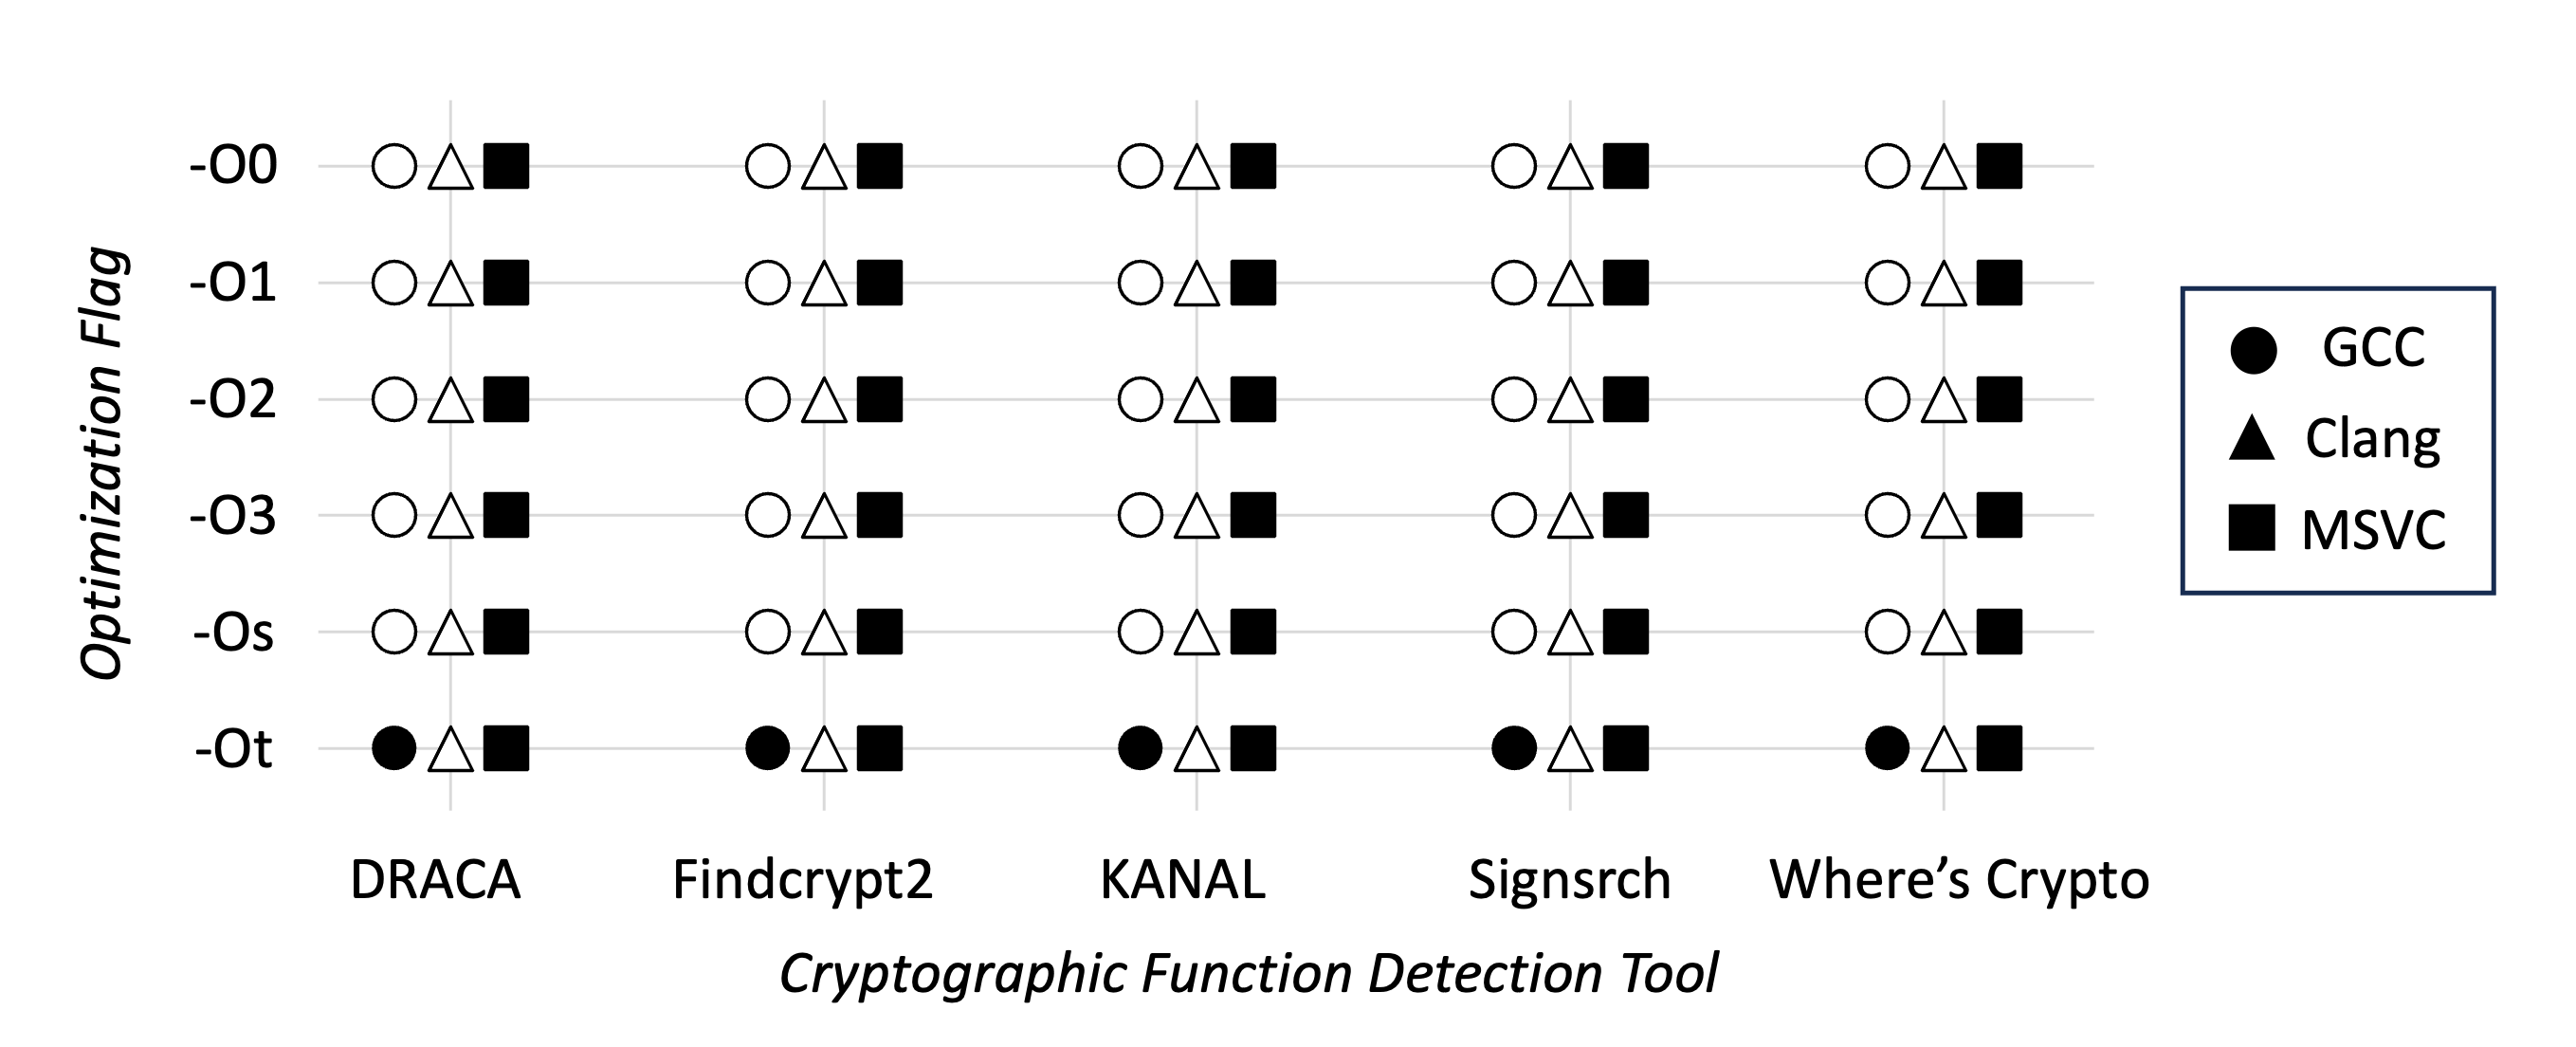
\includegraphics[width=0.8\linewidth,keepaspectratio]{ch-cryptobinary/figure/evaluate_compiler_new.png}
	%\vspace*{-10pt}
  \caption{Evaluation result for MD5 with different compilers. A full marker indicates that function can be detected and an empty marker that it cannot.}
  \label{fig:cryptobinary-evaluate_compiler}
\end{figure}

\fanyo{fix typo in figure!!!}

In this example, DRACA, Findcrypt2, PEiD KANAL, Signsrch, and Where's Crypto support detecting the MD5 algorithm. However, their detection capabilities are influenced by the compiler used. All of these tools can detect the MD5 algorithm in binaries compiled with the MSVC compiler, regardless of the optimization flag. In contrast, for binaries compiled with GCC, they can only detect the MD5 algorithm when the -O0 optimization flag is applied. Furthermore, when using the Clang compiler, none of these tools were able to detect the MD5 algorithm in the binary. This suggests that differences between compilers may significantly impact a tool's analysis results. In general, we found that the MSVC compiler has less impact on detection results compared to GCC and CLANG. Specifically, if a tool can detect a certain cryptographic algorithm in a program compiled by GCC or CLANG, it will also be able to detect that algorithm in the same program compiled by MSVC.

For example, Signsrch shows inconsistent performance with Clang, GCC, and MSVC, identifying the SHA-1 hash function in certain programs compiled with identical optimization flags but using a different compiler. We also observe same behaviour for DARACA when detect XXTEA algorithm (see Table \ref{tab:cryptobinary-benchmarks} for details).

The structure of binaries produced by different compilers, such as MSVC, GCC, and LLVM, can vary significantly due to differences in object file formats, optimization strategies, and code generation techniques. Binary analysis often relies on symbolic information, padding, and inlined data, all of which are heavily influenced by the compiler version~\cite{andriesse2017compiler}. These variations can hinder the effectiveness of cryptographic function detection tools, potentially leading to inaccurate or incomplete detection results.

%\noindent\fbox{%
    %\parbox{\textwidth}{%
        %Future Research Question: At present, it is notable that none of the cryptographic function detection tools take into account the influence of the compiler. Our evaluation results have revealed that the choice of compiler plays a pivotal role in cryptographic function analysis.
        %%We have identified differences in behavior between standard, widely used compilers like GCC and CLANG. Additionally, other non-standard compilers may introduce even more variations and challenges for cryptographic function detection tools. 
        %The exploration of compiler effects and their incorporation into cryptographic function detection tools represents an enticing avenue for future research, and understanding and accounting for these compiler-related influences could significantly enhance the accuracy and reliability.
    %}%
%}

\begin{takeaway}
\textbf{Future Research:} At present, it is notable that none of the cryptographic function detection tools consider the impact of the compiler. Our evaluation results have revealed that the choice of compiler plays a pivotal role in cryptographic function analysis.
        %We have identified differences in behavior between standard, widely used compilers like GCC and CLANG. Additionally, other non-standard compilers may introduce even more variations and challenges for cryptographic function detection tools. 
        The exploration of compiler effects and their incorporation into cryptographic function detection tools represents an enticing avenue for future research.
        Moreover, understanding and accommodating these compiler-related influences could significantly enhance both accuracy and reliability.
        %and understanding and accounting for these compiler-related influences could significantly enhance accuracy and reliability.
\end{takeaway}


% \begin{table}[h]
% \centering
% \begin{tabular}{|cc|c|c|c|c|}
% \hline
% \multicolumn{2}{|c|}{Binary Prog}                    & DRACA  & Findcrypt2 & PEiD KANAL & Where's Crypto \\ \hline
% \multicolumn{1}{|c|}{\multirow{2}{*}{XXTEA}} & gcc   & \cellcolor{gray!25}\cmark & \cmark     & \cmark     & \cmark         \\ \cline{2-6} 
% \multicolumn{1}{|c|}{}                       & clang & \cellcolor{gray!25}\xmark & \cmark     & \cmark     & \cmark         \\ \hline
% \multicolumn{1}{|c|}{\multirow{2}{*}{MD5}}   & gcc   & \cellcolor{gray!25}\cmark & \cellcolor{gray!25}\cmark     & \cellcolor{gray!25}\cmark     & \cellcolor{gray!25}\cmark         \\ \cline{2-6} 
% \multicolumn{1}{|c|}{}                       & clang & \cellcolor{gray!25}\xmark & \cellcolor{gray!25}\xmark     & \cellcolor{gray!25}\xmark     & \cellcolor{gray!25}\xmark         \\ \hline
% \end{tabular}
% \caption{Untitled}
% \label{tab:evaluate_compiler}
% \end{table}

 %\begin{table}[h]
 %\centering
 %\begin{tabular}{|c|c|c|c|c|c|c|c|c|c|c|c|c|}
 %\hline
 %Flag   & None  & -O0   & -O1   & -O2   & -O3   & -Os   & -Ofast & obs\_sub & obs\_fla & obs\_bcf & Multi\_flag 1 & Multi\_flag 2 \\ \hline
 %Prog 1 & \cmark & \cmark & \cmark & \xmark & \xmark & \xmark & \xmark  & \cmark    & \cmark    & \cmark    & \cmark         & \xmark         \\ \hline
 %Prog 2 & \cmark & \cmark & \xmark & \xmark & \xmark & \xmark & \xmark  & \cellcolor{gray!25} & \cellcolor{gray!25} & \cellcolor{gray!25} & \cellcolor{gray!25} & \cellcolor{gray!25} \\ \hline
 %\end{tabular}
 %\caption{Untitled}
 %\label{tab:evaluate_flag}
 %\end{table}

\subsection{Impact of Optimization Flags}
%\emph{R2: Is there any impact from optimization flags?}

Optimization flags and obfuscation can significantly impact the analysis results for cryptographic functions \cite{ren2021unleashing}. CryptoHunt\cite{xu2017cryptographic} and FALKE-MC \cite{aigner2018falke} have explored this direction. CryptoHunt primarily focuses on specific optimization flags such as \texttt{-O0}, \texttt{-O1}, and \texttt{-O2}, while FALKE-MC includes programs compiled with \texttt{-Os} and \texttt{-Ofast} for training. However, we are unable to run either of these tools, so we cannot confirm their detection performance with optimization/obfuscations flags. In order to comprehensively investigate this topic, we have expanded our study to include additional optimization flags, obfuscation techniques, and their combinations, thereby providing a more thorough exploration of their impact on cryptographic algorithm detection.

Our findings indicate that both optimization flags and obfuscations can affect detection capability. For instance, based on our results in \autoref{tab:cryptobinary-benchmarks}, we can see that Findcrypt2, PEiD KANAL, Signsrch, and Where's Crypto can detect MD5 when compiled without optimization/obfuscation flags or compiled with \texttt{-O1}. However, none of these tools can detect MD5 if the binary program is compiled with advanced optimization/obfuscation flags such as \texttt{-O2}, \texttt{-Ofast}, or \texttt{-obs\_sub}. In addition, we observed that Signsrch exhibits inconsistent performance for SHA-1 or SHA-256, and DRACA shows unstable performance with XTEA and XXTEA when running with optimization or obfuscation flags.
Optimization flags significantly alter the structure and behavior of a binary program by improving performance, reducing size, and modifying control flow. Techniques like function inlining, loop unrolling, and dead code elimination obscure the original source code structure, making it more difficult for analysts to identify cryptographic functions.
% Table \ref{tab:evaluate_flag} shows selected evaluation results of Signsrch with two different experiment. Experiment 1 is a program contains the SHA-1 hash function compiled by CLANG with different optimization flags or obfuscations, while experiment 2 contains the MD5 hash function compiled by GCC with different optimization flags (as the GCC compiler does not support obfuscations).

% \begin{table}[h]
% \vspace*{-6pt}
% \centering
% \footnotesize
% \begin{tabular}{|c||c|c|c|}
% \hline
% Flag          & SHA-1        & MD5                 \\ \hline \hline
% None          & \cmark       & \cmark              \\ \hline
% -O0           & \cmark       & \cmark              \\ \hline
% -O1           & \cmark       & \xmark              \\ \hline
% -O2           & \xmark       & \xmark              \\ \hline
% -O3           & \xmark       & \xmark              \\ \hline
% -Os           & \xmark       & \xmark              \\ \hline
% -Ofast        & \xmark       & \xmark              \\ \hline
% obs\_sub      & \cmark       & \cellcolor{gray!25} \\ \hline
% obs\_fla      & \cmark       & \cellcolor{gray!25} \\ \hline
% obs\_bcf      & \cmark       & \cellcolor{gray!25} \\ \hline
% -obs\_sub, obs\_fla, obs\_bcf & \cmark       & \cellcolor{gray!25} \\ \hline
% -obs\_sub, obs\_fla, obs\_bcf, -O3 & \xmark       & \cellcolor{gray!25} \\ \hline
% \end{tabular}
% %}
% \caption{Evaluation results of Signsrch with different optimization flags}
% \label{tab:evaluate_flag}
% \vspace*{-0.6cm}
% \end{table}

% We discovered that both optimization flags and obfuscations can affect detection, potentially resulting in false negatives (where the binary contains a cryptographic algorithm but the tool cannot detect it). For example, Signsrch successfully detects TEA in Program 1 compiled without any optimization flags or obfuscations. However, with additional optimization flags, Signsrch cannot detect any cryptographic algorithms at all anymore, resulting in false negatives.

% Meanwhile, Signsrch successfully detects MD5 in Program 2 compiled with no optimization flags or -O0, but cannot detect MD5 in the binary compiled with any other optimization flags or obfuscations. We observed the same results when detecting MD5 with other tools. Therefore, we conclude that current cryptographic detection tools may not be able to handle some algorithms, like MD5, if the binary is compiled with advanced optimization flags such as $-O3$.

%\noindent\fbox{%
    %\parbox{\textwidth}{%
        %Future Research Question: Optimization and obfuscation have been noticed by some researchers such as CryptoHunt, a cryptographic detection tool designed for obfuscated binaries. However, the limitation of CryptoHunt, such as slow time performace due to the large trace size, may reduce its applicability such as large scale project.  Given that certain other tools struggle to handle obfuscated binaries in certain algorithms,  we maintain that the exploration of optimization and obfuscation remains an interesting and important future research direction.
    %}%
%}

\begin{takeaway}
\textbf{Future Research:} The effects of optimization and obfuscation have been noted in works such as CryptoHunt, which is designed specifically for obfuscated binaries. However, limitations such as slow performance due to the large trace size, may reduce its applicability for large scale projects. Considering that many tools seem to face challenges with obfuscated binaries, we assert that investigating the effects of optimization and obfuscation continues to be a compelling and critical avenue for future research.
\end{takeaway}

% \begin{figure}
% \centering
% \begin{minipage}{.45\textwidth}
%   \centering
%   \includegraphics[width=\linewidth]{./images/evaluate_algo.jpg}
%   \caption{Untitled}
%   \label{fig:evaluate_algo}
% \end{minipage}%
% \qquad
% \begin{minipage}{.45\textwidth}
%   \centering
%   \includegraphics[width=1.15\linewidth]{./images/evaluate_tool.jpg}
%   \caption{Untitled}
%   \label{fig:evaluate_tool}
% \end{minipage}
% \end{figure}

\subsection{Impact of Different Algorithm Versions}
\label{subsec:cryptobinary-algo-version}
% \begin{figure}[ht]
%   \includegraphics[width=\columnwidth,keepaspectratio]{./images/evaluate_nonstandard.jpg}
%   \caption{Untitled}
%   \label{fig:evaluate_nonstandard}
  
% \end{figure}

%\emph{R5: Is the version of the algorithm significant during detection?}

We also carried out evaluations to determine whether variations in a cryptographic algorithm affects the success of its detection. As a case study, we analyzed different variants of the Tiny Encryption Algorithm (TEA), including standard TEA, XTEA, and XXTEA. While all the tools were able to successfully detect TEA binaries with any of these three variants, we observed some interesting details in the detection results.

\begin{table}[h]
%\vspace{-6pt}
\centering
\begin{tabular}{l||l|l}
\hline
Algorithm & DRACA                                                                      & Signsrch                                                                                   \\ \hline \hline
TEA   & \begin{tabular}[c]{@{}l@{}}* RC5 or RC6 - 50\%\\ ** TEA - 67\%\end{tabular} & \begin{tabular}[c]{@{}l@{}}* TEA1\_DS {[}32.le.4{]}\\ ** TEA encryption/decryption\end{tabular} \\ \hline
XTEA  & \begin{tabular}[c]{@{}l@{}}* RC5 or RC6 - 50\%\\ ** TEA - 34\%\end{tabular} & * TEA1\_DS {[}32.le.4{]}                                                                     \\ \hline
XXTEA & \begin{tabular}[c]{@{}l@{}}* RC5 or RC6 - 50\%\\ ** TEA - 67\%\end{tabular} & * TEA1\_DS {[}32.le.4{]}                                                                     \\ \hline
\end{tabular}
%}
\caption{Output when evaluating DRACA and Signsrch with different variants of TEA}
\label{tab:cryptobinary-evaluate_variant}
%\vspace*{-0.7cm}
\end{table}

For example, as shown in Table \ref{tab:cryptobinary-evaluate_variant}, when using DRACA to analyze binaries containing TEA or XXTEA, the tool provides a confidence score. It tends to determine that a binary program is more likely to contain TEA functions if TEA or XXTEA is present. However, when analyzing binary programs containing XTEA, DRACA may incorrectly identify RC5 or RC6 as being present in 50\% of cases, and TEA functions in only 34\% of cases. In contrast, Signsrch is able to detect TEA functions in all three binary programs containing TEA, XTEA, or XXTEA, but it may identify different TEA signatures in each binary.

%\noindent\fbox{%
    %\parbox{\textwidth}{%
        %Future Research Question: Our evaluations suggests that the variant versions of cryptographic algorithms also play a crucial role in detection, and that cryptographic function detection tools may not be able to accurately detect certain variant algorithms based on their signatures alone. Currently, there is no approach focuses on this difference, which could be a future research path for crytpographic function detection.
    %}%
%}

\begin{takeaway}
\textbf{Future Research:} Our evaluations indicates that the variant or version of a cryptographic algorithm plays a crucial role in its detection, suggesting that existing tools might struggle to accurately identify certain variants based on their signatures alone. Currently, there is no approach that focuses on this difference, which could be an interesting future research path.
\end{takeaway}



\subsection{Impact of Intentional Evasion Tactics}
%\fanyo{Change title to Detect binary with malware or something similar?}
\label{subsec:cryptobinary-algo-version1}
%\emph{R6: Are ``malicious'' versions of cryptographic algorithms trickier to detect?}

We selected multiple (ransomware) malware binaries, including CryptoLocker \cite{hansberry2014cryptolocker}, CryptoWall \cite{cabaj2015network}, Locky \cite{locky}, TeslaCrypt \cite{lemmou2018infection}, and Win32Dircrypt \cite{win32dircrypt}, to evaluate if cryptographic detection tools are better or worse at finding cryptographic algorithms in malware binaries (where authors might intentionally try to obfuscate the presence of cryptography) versus normal applications. 

%The CryptoLocker ransomware is a trojan that targeted computers running Microsoft Windows via infected email attachments and encrypted certain types of files stored on local and mounted network drives. 
%Cryptowall operates as a ransomware virus that employs a Trojan horse to encrypt files on a compromised computer, demanding users to make a payment in exchange for a decryption key.
%Locky is ransomware malware that delivers malicious macros through Microsoft Word documents attached to emails.
%TeslaCrypt is a ransomware trojan that targets game-play data, with newer variants also affecting other file types \cite{GALLAGHER_2015}.  
%Win32Dircrypt may encrypt file through spam emails or by being downloaded by other malware and ask payment for decryption.

We tested the tools with these malware samples and present the results in Table \ref{tab:cryptobinary-evaluate_malware}. It is worth noting that malware may have different versions depending on the discovery date, and detection results are highly dependent on these versions. We found that the tools could detect cryptographic functions in TeslaCrypt version 2 but failed to do so in versions 1 and 3. This suggests that the malware may employ non-standard algorithms to evade binary analysis in certain versions, increasing the difficulty of detection. Furthermore, cryptographic functions in CryptoLocker's September 10, 2013 version were detectable by the tools, but in the November 20, 2013, and January 22, 2014 versions, they were no longer detectable. In the latter two versions, some tools identified the presence of anti-debugging techniques in the malware, which might explain why cryptographic functions could not be detected anymore.

%We found that none of the cryptographic detection tools we chose can detect AES in CryptoWall, since CryptoWall primarily uses RSA, and may only use non-standard versions of AES in its source code.
%Meanwhile, most tools cannot detect AES in TeslaCrypt, but DRACA successfully finds AES algorithm in TeslaCrypt version 3372C.  And even though AES cannot be detected, some tools still successfully found other cryptographic hash algorithms in CryptoWall and TeslaCrypt including SHA256, RIPEMD, and Fork256.


\begin{table}[h]
\vspace*{-0.1cm}
\centering
\begin{adjustbox}{max width=\textwidth}
\begin{tabular}{c||c|c|c|c}
\hline
Malware                 & DRACA  & PEiD KANAL  & Signsrch  & Note       \\ \hline 
\hline
CryptoLocker\_10Sep2013 & \xmark & \cmark      & \cmark    &            \\ \hline
CryptoLocker\_20Nov2013 & \xmark & \xmark      & \xmark    & anti-debug \\ \hline
CryptoLocker\_22Jan2014 & \xmark & \xmark      & \xmark    & anti-debug \\ \hline
CryptoWall              & \xmark & \xmark      & \xmark    & anti-debug \\ \hline
Locky                   & \xmark & \xmark      & \xmark    &            \\ \hline
TeslaCrypt\_v1          & \xmark & \xmark      & \xmark    &            \\ \hline
TeslaCrypt\_v2          & \cmark & \cmark      & \cmark    &            \\ \hline
TeslaCrypt\_v3          & \xmark & \xmark      & \xmark    &            \\ \hline
Win32Dircrypt           & \xmark & \cmark      & \cmark    &            \\ \hline
\end{tabular}
%}
\end{adjustbox}
\caption{Evaluation results for cryptographic function detection in different malware versions}
\label{tab:cryptobinary-evaluate_malware}
%\vspace*{-0.6cm}
\end{table}


% \begin{table}[]
% \vspace*{-0.1cm}
% \centering
% \begin{tabular}{|l|c|c|c|}
% \hline
% Malware & DRACA & PEiD KANAL & Signsrch \\ \hline
% CryptoWall\_1002 & \Circle & \LEFTcircle & \Circle   \\ \hline
% CryptoWall\_1003 & \Circle & \LEFTcircle & \Circle \\ \hline
% TeslaCrypt\_3372C & \CIRCLE & \LEFTcircle & \LEFTcircle \\ \hline
% TeslaCrypt\_51B4E & \Circle & \Circle & \Circle \\ \hline
% TeslaCrypt\_E906F & \Circle & \Circle & \Circle \\ \hline
% \end{tabular}
% \caption{Evaluation results for different malware versions}
% \label{tab:evaluate_malware}
% \vspace*{-0.6cm}
% \end{table}

%\noindent\fbox{%
    %\parbox{\textwidth}{%
        %Future Research Question: Malware detection is a major application for cryptographic function detection, and based on our evaluation, current cryptographic detection tool may not be able to detect the crytpographic function in the malware. Other researcher also notice this issues, and for example, environment-sensitive malware is a threat to CryptoHunt, which may result in false negative. Therefore, cryptographic function detection in malware sould be a major future developement for this topic.
    %}%
%}

\begin{takeaway}
\textbf{Future Research:} Cryptographic function detection can be a useful component in identifying malware, and according to our investigation, current tools do not consistently detect cryptographic functions within the malware samples.  This challenge has been noted in other research as well, for example, CryptoHunt identified environment-sensitive malware as a potential source of false negatives in detection efforts. Therefore, cryptographic function detection primarily focused on targeting malware could be a highly relevant source of future research in this area.
\end{takeaway}

% \subsection{Other Evaluations}
% A single binary program may contain multiple cryptographic algorithms that can be detected by the tool. When testing DRACA with a TEA program without obfuscation, the tool identified multiple cryptographic algorithms. Specifically, DRACA detected 67\% of TEA, 50\% of RC5/RC6, and 23\% of SHA-1. Furthermore, Signsrch was able to recognize the bzip2 binary due to the specific signature that Signsrch supports.



%%%%%%%%%%%%%%%%%%%%
\section{Discussion}
\label{sec:cryptobinary-discussion}

We now provide a discussion backed by our evaluation results and examination of existing work and implemented tools, delving into broader issues that we discovered.  This includes discussing additional overarching future research directions and key areas where improvements can be made moving forward.

%Within this particular section, we aim to delve deeper into the issues and potential avenues for further research that we have identified based on our comprehensive evaluation results. With consideration of the evaluation results, we found our some issues to detect cryptographic function in binary. Meanwhile, we have discovered several key areas where improvements could be made.


\subsection{Approaches to Algorithm Detection in Tools}

%\emph{R4: Can the same tool perform similarly well across different algorithms?}
% \begin{figure}[h]
%   \includegraphics[width=0.5\linewidth,keepaspectratio]{./images/evaluate_tool.jpg}
%   \caption{Untitled}
%   \label{fig:evaluate_tool}
  
% \end{figure}

We start by discussing the detection results of a single tool for different algorithms. We opted to evaluate 12 distinct algorithms (AES, DES, ECC, MD5, RC4, RC5, RSA, SHA-1, SHA-256, TEA, XTEA, and XXTEA) along with our microbenchmarks, various libraries, and a large-scale project.

Based on our evaluation (see \autoref{tab:cryptobinary-benchmarks}), we found that PEiD KANAL, SignSrch, and Where's Crypto can detect most algorithms we selected. This was somewhat expected as Where's Crypto is a more modern detection tool. HCD demonstrated average performance in our evaluation results.
%but it is the only tool that can detect ECC. 
Nonetheless, we came across cases where tools did not detect cryptographic functions they were expected to identify, indicating potential need to enhance detection accuracy.

\begin{takeaway}
\textbf{Future Research:} Current tools seemingly employ various (often distinct) approaches compared to one another. Many of these tools also provide developers with the opportunity to expand and enhance their detection capabilities. Therefore, future research could focus on improving existing technologies within individual tools and existing approaches to achieve broader applicability with higher detection rates, and to make it so that users do not need to use different tools to best identify different algorithms.
\end{takeaway}

\subsection{AI/ML Approach}
Artificial intelligence and machine learning (AI/ML) have been extensively applied across various domains to address complex problems. Previous works, like CryptoKnight, have utilized machine learning techniques for cryptographic function detection. However, in our evaluation, we found that these tools did not exhibit satisfactory performance. We attribute this issue not to the approach itself, but rather to the fact that these tools typically only offer a demonstration to showcase the potential application of AI/ML in this field. The main problem lies in the lack of sufficient signatures or analysis provided by these tools, which is likely the primary reason for their low performance.
\begin{takeaway}
\textbf{Future Research:} 
While current AI/ML based tools demonstrate the feasibility of utilizing AI/ML in cryptographic function detection, they fall short in providing the robust and comprehensive signature or analysis capabilities necessary for accurate detection.  These seem like promising future research directions.
\end{takeaway}

\subsection{Lack of Support for Modern Cryptographic Algorithms}

Many modern cryptographic algorithms, such as general Elliptic-Curve Cryptography (ECC) and more specifically ECDSA and ECDHE, have found widespread use in diverse applications~\cite{harkanson2017applications} due to their advantages in terms of smaller private key size and improved efficiency at equivalent or higher security levels. ECDSA is utilized in a number of areas, including electronic healthcare, banking, commerce, and vehicles \cite{al2019efficient}, and is currently supported by most major libraries, including cryptlib, Crypto++, libgcrypt, LibreSSL, and OpenSSL.
However, our evaluation reveals that existing work lacks the ability to find such modern algorithms. As such, this could be a rich area for future development and improvement. 
\begin{takeaway}
\textbf{Future Research:} 
As the prevalence of applications adopting ECC continues to rise, the ongoing development of cryptographic function detection has led to a disconnect between the outcomes of these efforts and the real-world applications that people are eager to test, leading to an important direction for future research.
\end{takeaway}

% Besides the evaluation metrics we evaluated in Section \ref{subsec:metrics} The false positive may affected by the 
% This underscores the importance of recognizing that the implementation of cryptographic functions can significantly impact detection ability. The presence of optimizations or deviations from the standard algorithm can also lead to false negatives in the detection process.
\subsection{Comparative Detection of Similar Algorithms Across Various Tools}
% \begin{figure}[h!]
%   \includegraphics[width=0.5\linewidth,keepaspectratio]{./images/evaluate_algo.jpg}
%   \caption{Untitled}
%   \label{fig:evaluate_algo}
%\emph{R3: Are some algorithms easier to detect compared to others?}

% \end{figure}
Our evaluation helps provides insights from an algorithmic perspective on how well different tools can detect the same cryptographic algorithm. In our evaluation, we test the tools' abilities to find cryptographic functions in different settings (optimization flags, compilers, etc.). \autoref{fig:cryptobinary-algo_easy} shows the percentage of algorithms that can be successfully detected by a tool across all evaluation experiments that we ran.
We can see that TEA, RC5, and SHA can be successfully detected in most experiments. However, AES, and MD5 can only be found in a few experiments, with algorithms like RC4 and ECC not even being detected at all.

\begin{figure}[t]
    \centering
  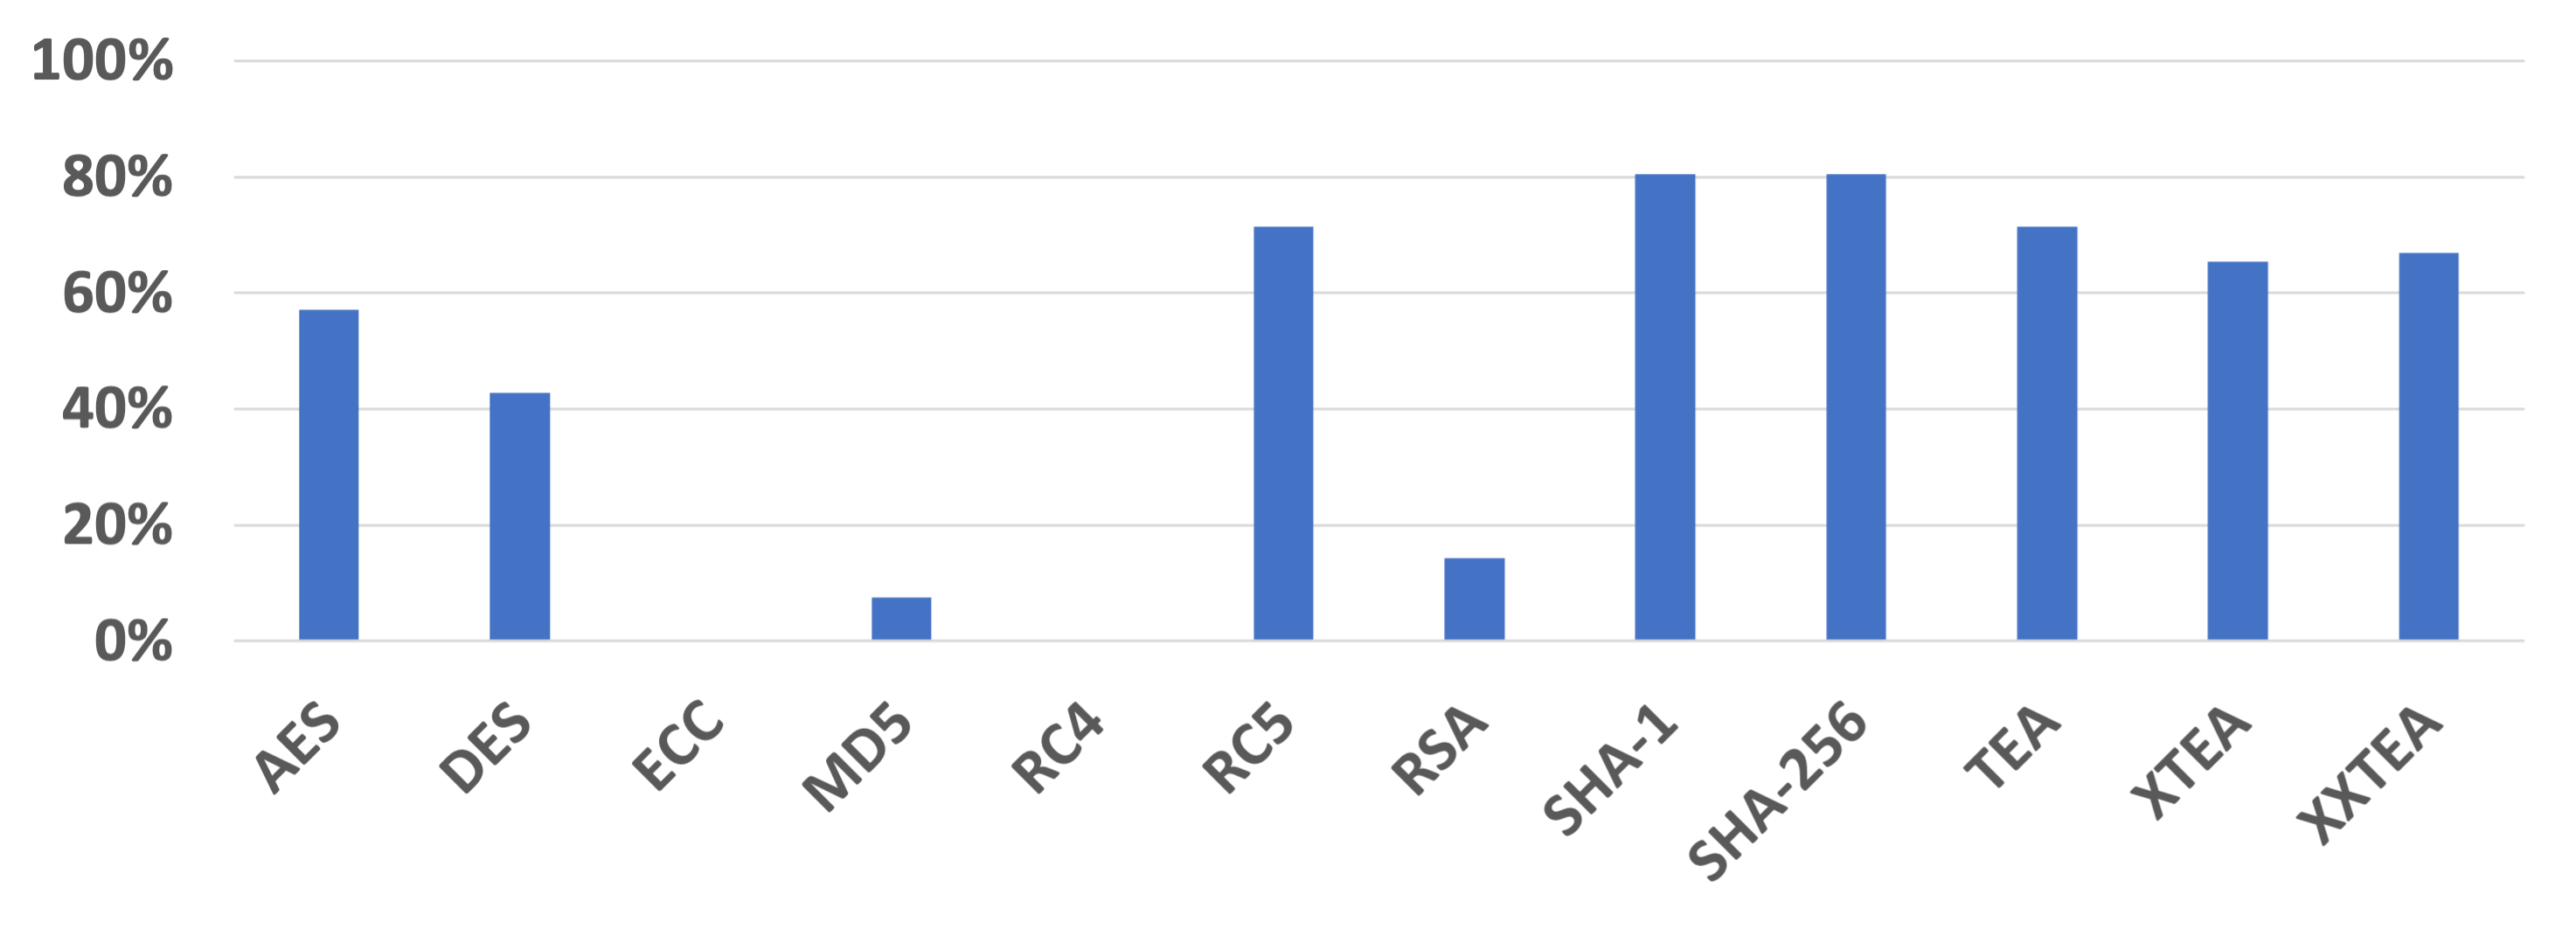
\includegraphics[width=0.95\linewidth,keepaspectratio]{ch-cryptobinary/figure/algoeasy.png}
  \caption{Detection percentage by algorithm across all tools}
  \label{fig:cryptobinary-algo_easy}
\end{figure}

From our observations, it is not evident that there exists a consistent rule governing the ease of detecting specific categories of cryptographic functions. For instance, when considering two hash functions, MD5 and SHA, we note markedly different results. Even within the same family we find variations; TEA and RC5, both belonging to the block cipher family, exhibit detectability, while DES, another block cipher, proves more challenging to detect.

%\noindent\fbox{%
    %\parbox{\textwidth}{%
        %Future Research Question: Some cryptographic algorithms are more challenging to detect than others, as indicated by our evaluation results. Notably, we have not observed a distinct pattern suggesting that algorithms within a specific category consistently present greater difficulty in detection. Therefore, the future research could focus on how to detect cryptographic algorithms that appear to be harder to identify or investigate the underlying factors that contribute to variations in the detectability of algorithms within the same category.
    %}%
%}

\begin{takeaway}
\textbf{Future Research:} Some cryptographic algorithms appear to be more challenging to detect than others. However, we have not observed a distinct pattern suggesting that algorithms within a specific category consistently present greater difficulty in detection. Therefore, future research could focus on how to detect cryptographic algorithms that appear to be harder to identify or investigate the underlying factors that contribute to variations in the detectability of algorithms within the same class.
\end{takeaway}



%\subsection{Leveraging General Binary Analysis Techniques}
%\label{leverage-binary}
%%\noindent\fbox{%
    %%\parbox{\textwidth}{%
        %%Future Research Question: 
    %%}%
%%}
%Binary code similarity analysis is an active area of research in the software community. There has been a plethora of research~\cite{david2017similarity, saebjornsen2014detecting, liu2018eclone, chandramohan2016bingo, mckee2019software, ding2019asm2vec, ming2017binsim, xu2017neural} to compare two or more binaries to identify their similarities or variances.  
%
%BLEX~\cite{egele2014blanket} proposed a dynamic similarity testing system based on the novel technique of blanket execution 
%consisting of seven binary code semantics extractor. Tinbergen~\cite{mckee2019software} presented a framework which infers function semantics through program state change. DyCLINK~\cite{su2016code} used dynamic dependency graph to capture code behavior at the instruction level and then
%performed similarity analysis via computing an isomorphism between sub graphs.
%There are also some notable NLP based binary similarity analysis techniques~\cite{ding2019asm2vec, xu2017neural}.
%Asm2Vec~\cite{ding2019asm2vec} is a representation learning model that learns latent lexical semantics between
%tokens and represents an assembly function as an internally weighted mixture of collective semantics.
%Gemini~\cite{xu2017neural} proposes a neural network-based approach to compute the embedding, i.e., a numeric vector, based on the control
%flow graph of each binary function and then performs the similarity detection via measuring the distance between the embeddings for two functions.

%\begin{takeaway}
%\textbf{Future Research:}
%Although binary similarity research is very similar to some cryptographic function identification approaches and shares a similar set of challenges, cryptographic detection research has a much more limited scope of work and techniques thus far.
%Hence, an avenue for future research is investigating the use of binary similarity techniques in this more targeted space.  
%\end{takeaway}


% \subsection{Discussion of Evaluation Results}
% Based on our evaluation, we found that most of the cryptographic detection tools have similar performance such as

% \begin{itemize}[leftmargin=*]
%     \setlength{\itemsep}{0pt}
%     \setlength{\parskip}{0pt}
%         \item Cannot detect RSA and modern cryptohtrapicy algorithm ECC in binary
%         \item Optimization flag and compiler do not affect the detetcion results in SHA (except for Signsrch) and TEA
%         \item Can only detect MD5 compiled with no flag or $\O0$ in GCC
% \end{itemize}

% In the course of our evaluation, we have encountered instances of false negatives in certain cryptographic detection tools. For instance, both DRACA and FindCrypt2 assert their ability to detect DES functions within binaries. However, we were unable to replicate this result even when using a standard DES implementation without any obfuscation during compilation.

\subsection{User Experience}

Considering the experience and insights we have garnered from our evaluation process, we believe that discussing the developer experience is also an intriguing topic, in terms of how developers interact with these tools and their ease of use.

Older cryptographic detection tools, such as DRACA, PEiD KANAL, and SignSrch, do not require developers to compile and build the tools from source code. Developers can readily utilize these tools with supported operating systems. However, when compared to some better performing tools, these user-friendly alternatives exhibit lower performance and utility. For example, obfuscation can disturb the binary analysis process of Signsrch, leading to false negatives in the detection of certain cryptographic algorithms. Furthermore, DRACA struggles to accurately analyze packed executable programs, and consequently, it can only provide a rudimentary analysis outcome, despite its ease of use.

In addition to the aforementioned challenges, some tools pose difficulties for users due to technological complexity or data-related issues. Take, for instance, IDA Scope, Findcrypt2, and Where's Crypto, which all rely on IDA Pro. IDA Pro is not a free, open-source software, and these tools cannot be utilized by developers without it. Conversely, tools such as CryptoKnight and other machine learning-based techniques require users to provide substantial amounts of data, which further compounds the difficulty of using these tools. 

However, these tools generally exhibit superior performance when compared to user-friendly alternatives. For instance, CryptoHunt consistently yields accurate analysis results for identification within obfuscated programs. Where's Crypto, one of the most recent cryptographic detection tools, broadens the scope of analysis to encompass unfamiliar and proprietary cryptographic primitives, without relying on heuristics to select code fragments.

\subsection{Challenges for Future Research}
\label{subsec:cryptobinary-challenges}

%Identifying cryptographic functions has its own sets of challenges. 
Based on our evaluation, we have identified several challenges that make cryptographic function identification difficult.
In this subsection, we discuss some of these challenges, as we believe they may help inform future tool development and areas of research.

%%%%%%%%%%%%%%%%%%%%%%%%
\parhead{Obfuscation.} One of the major challenges in cryptographic function identification is obfuscation.
The initial purpose of obfuscation was to protect software intellectual
property~\cite{collberg1997taxonomy} from malicious reverse engineering
attempts. However, malware authors adopted obfuscation techniques as a way to
avoid detection. Various types of obfuscation techniques have been implemented
to thwart any form of detection. These obfuscation techniques can be primarily
categorized as: control-flow obfuscation, data obfuscation, and layout obfuscation.
For a variety of reasons, one might still wish to identify cryptographic code
even in the face of such obfuscation techniques, particularly given its prevalence nowadays.
%Malware authors mostly adhere to control-flow and data obfuscations.

Control-flow obfuscation is the most common type of obfuscation. A control-flow graph (CFG) \cite{CFG} embodies the graphical
representation of the flow of a program. To hinder CFG-based detection, malware authors introduce techniques such as including bogus control-flow \cite{li2021code}, control-flow flattening \cite{cfg_f}, and opaque predicates \cite{xu2018opaque}. 
Similar to control flow obfuscation, data obfuscation techniques, like data aggregation and data
splitting, attempt to hinder approaches based on input/output relationships. For example, one might split a single variable into two to prevent detection.
%\autoref{lst:data_splitting} shows an example of data
%obfuscation, and how one variable used in \autoref{lst:normal_program}
%can be split into two variables to prevent detection.  
%
%\lstset{language=C,
        %label=lst:normal_program,
        %float=h,
        %caption={Normal program},
        %captionpos=b,
        %showlines=true,
        %breaklines=true,
        %breakatwhitespace=true,
        %tabsize=2,basicstyle=\footnotesize}
%\hspace*{-1.1cm}
%\begin{lstlisting}
%int var1 = func1();
%int var2 = func2();
%
%while(condition statement) {
	%int p1 = var1 * var2;
	%int p2 = var1 + var2;
%}
%\end{lstlisting}%
%%\hfill
%%\hspace*{0.1cm}
%\vspace{5pt}
%
%\lstset{language=C,
        %label=lst:data_splitting,
        %float=h,
        %caption={Data splitting},
        %captionpos=b,
        %breaklines=true,
        %breakatwhitespace=true,
        %tabsize=2,basicstyle=\footnotesize}
%\begin{lstlisting}
%int var1 = func1();
%int var2 = func2();
%
%short var11 = (short) (var1 >> 16);
%short var12 = (short) (var1 & 0xffff);
%
%while(condition statement) {
    %int new_var = (int) ((var11 << 16) | (var12 & 0xffff););
%
    %int p1 = new_var * var2;
    %int p2 = new_var + var2;
%}
%\end{lstlisting}
Layout obfuscation~\cite{xu2020layered} scrambles the layout of a program's instructions while keeping the original syntax intact. Layouts can be obfuscated by adding meaningless classifiers, stripping redundant symbols, separating related code, as well as adding junk code.

%%%%%%%%%%%%%%%%%%%%%%%%%%%%%%%%%%%%%

\parhead{Implementation Variation.} Despite having a well-defined specification, cryptographic algorithms can be implemented in a number of
ways while still achieving the same result.  In addition, cryptography is not always implemented correctly or exactly to spec.
For example, buggy implementations of the TEA algorithm
were found~\cite{calvet2012aligot} in malware such as Storm Worm and Silent Banker.
Hence, even if a detection approach can find an ideal implementation of an algorithm, there is no
guarantee it can also detect all the implementation variations
of the same algorithm. 
%We believe it is valuable (but challenging) to be able to identify both intended implementation variations, as well as as incorrect (but close) ones.
Our evaluations in this space are discussed in \autoref{subsec:cryptobinary-algo-version} and \autoref{subsec:cryptobinary-algo-version1}.

%%%%%%%%%%%%%%%%%%%%%%%%%%%%%%%%%%%%%%%%%%%%%%%%%%%

\parhead{Differences in Cryptographic Functions.} There are fundamental differences in different classes of cryptographic algorithms.
Cryptographic features (see \autoref{sec:cryptobinary-features}) present in one algorithm may not be present in others.
For instance, the data avalanche effect~\cite{li2012cipherxray} which says that an insignificant change in the input parameters can
make significant differences in the output, works well for identifying block ciphers. In the case of stream ciphers, there are
no such observations like data avalanching. Tools must be designed to account for these differences if they wish to identify broad classes of algorithms.

%%%%%%%%%%%%%%%%%%%%%%%%%%%%%%%%%%%%%%%%%%%%%%%%%%%

\parhead{Compilers.} The choice of compiler can significantly impact the binary structure of a program in various ways such as format, linking, inline functions, and compatibility with different architectures. The incorporation of anti-analysis techniques further adds to the complexity of cryptographic function detection. Consequently, working with different compilers can introduce numerous challenges. 
%Possessing knowledge about compiler behavior becomes essential for reverse engineers, security analysts, and detection tools to effectively identify cryptography within a binary program.
Our study (Section \ref{subsec:cryptobinary-effect-compiler}) demonstrates how a tool's detection capabilities can vary greatly depending on the compiler used.


%%%%%%%%%%%%%%%%%%%%%%%%%%%%%%%%%%%%%%%%%%%%%%%%%%%
\parhead{Comparison to General Binary Analysis.}
Binary code similarity analysis is an active area of research in the software community. There has been a plethora of research~\cite{david2017similarity, saebjornsen2014detecting, liu2018eclone, chandramohan2016bingo, mckee2019software, ding2019asm2vec, ming2017binsim, xu2017neural} to compare two or more binaries to identify their similarities or variances.  
While such generic binary analysis techniques can be leveraged in the detection of cryptographic functions, future researchers should bear in mind that detecting cryptographic functions in binary code remains a multifaceted challenge. Cryptographic algorithms exhibit significant variability in terms of complexity and implementation. They often involve intricate mathematical operations and employ various techniques such as bit manipulation, modular arithmetic, and logical operations. This complexity can pose difficulties in identifying cryptographic functions without specific knowledge of the algorithm being utilized.
%Furthermore, unlike some other types of functions or libraries that may have standardized signatures or calling conventions, cryptographic functions may lack easily recognizable patterns or signatures. They can be 
In addition, they can be implemented in diverse ways and may not adhere to consistent naming or calling conventions, rendering them more challenging to identify through static analysis alone.

%Additionally, detecting cryptographic functions in binary code constitutes a specialized domain within general binary analysis. Consequently, we anticipate a higher level of accuracy compared to detecting other types of functions in binary code.


%%Where's crypto, one of the latest cryptographic detection tool developed in 2021, provides an novel approach combines subgraph isomorphism with symbolic execution to find cryptographic algorithm in binary, but we did not discover a major performance improvement according to our evaluation results.


\section{Conclusion}

Cryptographic function identification has been a popular area of study in both academia and industry. However, we noticed a lack of consistent means for evaluation and comparison among tools.
As such, in this work we conduct comprehensive reproduction and replication studies on all existing work in the space.
To complement the traditional R+R studies, we developed a comprehensive testing and evaluation framework which includes a number of modern cryptographic algorithms and real world examples, that allow for the comparison of both existing and future work in a uniform manner.
Finally, we highlight major gaps in existing work, especially as they relate to modern cryptographic primitives and real-world use cases,
and discuss a variety of important avenues for future work.